%==============================================================================
%  MATH 231 -- Linear Algebra I (Queens College, Fall 2026)
%  MATRIX UNIT, PART 1 -- Linear Systems and the Matrix
%
%  A NEW UNIT.  Section numbering restarts at 1 here.  It does NOT continue
%  from the vector unit (Sections 1-24) and is unrelated to the computational
%  unit, which also restarts at 1.  Consequently every cross-reference OUT of
%  this unit must name the unit explicitly ("the vector unit, Sec. 16.5"),
%  because a bare "Sec. 1.5" is now ambiguous three ways.  The front matter
%  states that convention for students.
%
%  STATUS: complete.  Sections 1-9.
%
%    Sec. 1-2   motivate the matrix from the coordinate problem and stop at
%               Vx = u.  (These came first and are unchanged.)
%    Sec. 3-9   step back and define the matrix in general: what it is, what
%               shapes exist, and the operations on it.
%
%  SEC. 9 (TRACE) SITS AFTER MULTIPLICATION deliberately.  The trace could be
%  defined as soon as Sec. 3 -- it needs only the diagonal -- but placing it
%  after Sec. 8 buys tr(AB) = tr(BA), which is the one non-obvious fact about
%  it and which pairs directly against Sec. 8.4's warning that AB and BA differ.
%  The example reuses Example 8.3's matrices so the 2x2 and the 3x3 can be seen
%  agreeing on 212.
%
%  HOW to solve a system -- elimination, pivoting, existence and uniqueness --
%  is the announced sequel and is deliberately NOT begun here.  The closing
%  Looking-ahead in Sec. 8.6 flags it, and Sec. 4.4 plants the hint that the
%  method works by making the matrix triangular.
%
%  ORDER OF SEC. 7 AND 8 is deliberate and slightly unusual: inner and outer
%  products come BEFORE matrix multiplication is defined.  This is not an
%  oversight.  Sec. 7.1 multiplies a 1xn by an nx1, which introduces the
%  row-times-column atom on the smallest possible case, and Sec. 8.1 then opens
%  by saying matrix multiplication IS that atom applied to every (row, column)
%  pair.  It makes the rule feel derived rather than decreed, which matters
%  because no motivation for the rule is offered at this stage.  Do not reorder
%  these two sections without replacing that bridge.
%
%  CORRECTION against the drafted outline.  The outline said that R^(m x n) "is
%  formally called a field".  It is not one.  R is a field; R^(m x n) is merely
%  the SET of m x n real matrices, and it fails to be a field for a reason the
%  document can already state -- there is no general division by a matrix, and
%  by Sec. 8.4 multiplication does not even commute.  The outline's actual
%  intent (notation for "which set the matrices belong to", with the formal
%  definition of a field out of scope) is preserved exactly: Sec. 3.2 attaches
%  the word "field" to R where it belongs, defines R^(m x n) as a set, and adds
%  a short confusion box so no student carries away the wrong claim.
%
%  AUDIENCE: distributed to students.  Keep it free of instructor-facing
%  apparatus -- time budgets, pacing notes, teaching cues.
%
%  INDEX CONVENTION, the one decision this document turns on.  A basis vector
%  is written  v_i = [v_{1i}, v_{2i}, ..., v_{ni}],  so that
%
%        v_{ki}  =  the k-th component of the i-th basis vector
%                =  the entry of V in row k, column i.
%
%  FIRST index = row = which slot; SECOND index = column = which vector.  The
%  natural way to write it -- v_{ik} for "component k of vector i" -- reads the
%  indices in the opposite order from the matrix position, which forces the
%  reader to transpose mentally at every step of Sec. 2.  Sec. 1.3 states the
%  convention explicitly and Sec. 2.2 relies on it: with it, the (k,i) entry of
%  V is literally v_{ki} and no transposition is ever needed.
%
%  SEC. 2 IS DELIBERATELY SHORT.  It is the payoff of the whole document and
%  the place a reader is most likely to get lost, so it runs concrete-first:
%  the 3x3 example of Sec. 1.6 is carried through all four steps, and the
%  general n x n statement is only ever "the same thing, with dots".  Resist
%  adding intermediate notations here -- each extra layer between the system
%  and Vx = u costs more than it explains.
%
%  ROW VS COLUMN.  The vector unit writes vectors in row brackets, [v_1, v_2].
%  A matrix-vector product needs x as a column.  Sec. 2.3 has a flagged warning
%  reconciling the two: the bracket notation never asserted a shape, and the
%  two spellings denote the same vector.  Do not silently switch conventions
%  without that box, and do not "fix" the vector unit to use columns.
%
%  Compile with pdflatex (standard TeX Live packages only; uses tikz).
%==============================================================================
\documentclass[11pt]{article}

\usepackage[margin=1in]{geometry}
\usepackage{amsmath,amssymb,amsthm}
\usepackage[dvipsnames]{xcolor}
\usepackage{enumitem}
\usepackage{booktabs}
\usepackage{array}
\usepackage[hidelinks]{hyperref}
\usepackage{titlesec}
\usepackage{needspace}
\usepackage{tikz}
\usetikzlibrary{arrows.meta,decorations.pathreplacing}

%------------------------------------------------------------------ style ----
\titleformat{\section}{\large\bfseries\sffamily}{\thesection.}{0.6em}{}
\titleformat{\subsection}{\normalsize\bfseries\sffamily}{\thesubsection.}{0.5em}{}
\titlespacing*{\section}{0pt}{14pt}{6pt}

\theoremstyle{plain}
\newtheorem{thm}{Theorem}[section]

\theoremstyle{definition}
\newtheorem{defn}{Definition}[section]
\newtheorem{ex}{Example}[section]
\theoremstyle{remark}
\newtheorem*{rmk}{Remark}
\newtheorem*{warn}{A common confusion}

\newcommand{\lookahead}{\par\smallskip\noindent
  \textbf{\sffamily\textcolor{RoyalBlue}{Looking ahead.}}\ \ignorespaces}
\newcommand{\lookback}{\par\smallskip\noindent
  \textbf{\sffamily\textcolor{ForestGreen}{From the vector unit.}}\ \ignorespaces}

%--------------------------------------------------------------- notation ----
\newcommand{\R}{\mathbb{R}}
\newcommand{\vc}[1]{\mathbf{#1}}        % vectors: bold lower case
\newcommand{\mt}[1]{\mathbf{#1}}        % matrices: bold UPPER case
\newcommand{\norm}[1]{\lVert #1\rVert}
\newcommand{\proj}[2]{\operatorname{proj}_{#1}(#2)}
\newcommand{\comp}[2]{\operatorname{comp}_{#1}(#2)}
\newcommand{\bas}{\mathcal{B}}
\newcommand{\T}{^{\mathsf{T}}}          % transpose
\newcommand{\Z}{\mathbb{Z}}
\newcommand{\C}{\mathbb{C}}
\newcommand{\N}{\mathbb{N}}
\DeclareMathOperator{\spanop}{span}
\DeclareMathOperator{\diagop}{diag}

%------------------------------------------------------------- tikz helpers --
\tikzset{
  vecarr/.style   = {-{Stealth[length=2.6mm,width=2.0mm]},very thick},
  thinarr/.style  = {-{Stealth[length=2.2mm,width=1.7mm]},thick},
  axisline/.style = {->,gray!75,thin}
}
% \lattice{xmin}{xmax}{ymin}{ymax}
\newcommand{\lattice}[4]{%
  \draw[step=1cm,gray!25,very thin] (#1,#3) grid (#2,#4);
  \draw[axisline] (#1,0) -- (#2+0.45,0) node[right,font=\scriptsize,black]{$x$};
  \draw[axisline] (0,#3) -- (0,#4+0.45) node[above,font=\scriptsize,black]{$y$};
}

\title{\vspace{-1.2cm}\textbf{\sffamily MATH 231 -- Linear Algebra I}\\[4pt]
       {\large\sffamily The Matrix Unit, Part 1 \textbullet\ Linear Systems
        and the Matrix}\\[2pt]
       {\normalsize\sffamily Kiely Hall 326 \textbullet\
        Instructor: Kevin Bedoya}}
\author{}
\date{}

\begin{document}
\maketitle
\vspace{-1.6cm}

\noindent\textbf{About this document.} This opens the unit on \emph{matrices}.
It does not begin by defining one. It begins with a question the vector unit
left unanswered --- given a basis and a vector, how do you find the
coordinates? --- shows that the question is a system of $n$ linear equations,
and then builds the matrix as the notation that system demands.

\begin{warn}[Section numbers restart]
This unit numbers its sections from $1$ again. They do \emph{not} continue from
the vector unit, whose sections run $\S1$ to $\S24$, and they have nothing to do
with the computational unit, which also restarts at $1$. So a bare reference
such as ``\S1.3'' below means \S1.3 \emph{of this unit}. Whenever we point at
either of the other two we will name it, as in ``the vector unit, \S16.5''.
\end{warn}

\medskip
\noindent\textbf{Assumed from the vector unit.} $\R^{n}$ and the bracket
notation $\vc{v}=[\,v_1,\dots,v_n\,]$ (\S24.1); addition and scalar
multiplication (\S7--\S8); the dot product
$\langle\vc{u},\vc{v}\rangle=\sum_i u_iv_i$ (\S11.3); linear combinations and
span (\S16.2--\S16.3); coordinates and their uniqueness (\S16.4); the
coordinate problem for the standard basis (\S16.5); linear independence
(\S18.4); basis and dimension (\S16.3, \S17); and orthogonality (\S11.7).

\medskip
\noindent\textbf{What you should be able to do afterwards.} Say why a basis
turns ``find the coordinates of $\vc{u}$'' into a system of $n$ linear
equations in $n$ unknowns; write that system out from a given basis; say what
it means to solve it; recognise each equation as a dot product; build the
coefficient matrix $\mt{V}$ and the coordinate vector $\vc{x}$; state the
definition of a matrix--vector product and compute one; write a system as
$\mt{V}\vc{x}=\vc{u}$; and read that single equation in both directions ---
by rows as $n$ dot products, and by columns as one linear combination.
Then: define a matrix and address its entries; name the standard shapes and
patterns; add, scale and transpose matrices and recognise symmetry; write the
dot product, the outer product and the norm in transpose notation; multiply two
matrices and check in advance whether the product exists; and compute the trace
of a square matrix.

%==============================================================================
\section{The problem a basis leaves behind}
%==============================================================================
%------------------------------------------------------------------------------
\subsection{What a basis promises}
%------------------------------------------------------------------------------
Work in $\R^{n}$ and let
\[
  \bas = \{\,\vc{v}_1,\ \vc{v}_2,\ \dots,\ \vc{v}_n\,\}
\]
be a set of $n$ linearly independent vectors. That is enough to make $\bas$ a
basis.

\lookback Two facts do the work. A basis for $\R^{n}$ is a set that spans
$\R^{n}$ and is linearly independent (\S16.3), and a basis for $\R^{n}$ has
exactly $n$ vectors, since $\dim\R^{n}=n$ (\S17, \S24.1). What is not obvious is
that independence alone is enough --- that $n$ independent vectors cannot fail
to span. The vector unit proved this in $\R^{2}$ (\S18.5) and used it in
$\R^{n}$ (\S24.4). We take it as given.

\begin{rmk}
It is worth being clear that this is a genuine theorem and not a definition. In
principle a set could be independent and still miss part of the space; what the
result says is that in $\R^{n}$, once you have $n$ independent vectors, there is
no room left for it to miss anything. A proof in general dimension is one of the
things the machinery of this unit will eventually supply, which is a fair reason
to postpone it rather than assert it twice.
\end{rmk}

\noindent Being a basis, $\bas$ spans $\R^{n}$, and \emph{span} means exactly
what it said in the vector unit, \S16.3: the set of all linear combinations. So
every vector of $\R^{n}$ is reachable. Written out: for any $\vc{u}\in\R^{n}$
there are scalars $\alpha_1,\dots,\alpha_n\in\R$ with
\[
  \boxed{\;\vc{u}
  \;=\; \alpha_1\vc{v}_1 + \alpha_2\vc{v}_2 + \cdots + \alpha_n\vc{v}_n
  \;=\; \sum_{i=1}^{n}\alpha_i\vc{v}_i \;}
\]
and, because coordinates against a basis are unique (\S16.4), there is exactly
one such list of scalars.

That is a promise about existence, and it is the kind of promise that is easy to
undervalue. It says: pick any point of $\R^{n}$ you like --- any point at all,
however far out, in however many dimensions --- and it can be built out of these
$n$ vectors, in one and only one way.

What the promise does \emph{not} do is tell you the scalars.

%------------------------------------------------------------------------------
\subsection{The reverse problem}
%------------------------------------------------------------------------------
So we ask for them. This is the reverse problem of the vector unit, \S16.5, now
posed in $\R^{n}$ and against an arbitrary basis rather than the standard one:

\begin{quote}
Given a basis $\bas=\{\vc{v}_1,\dots,\vc{v}_n\}$ and a vector $\vc{u}\in\R^{n}$,
find the scalars $\alpha_1,\dots,\alpha_n$ with
$\vc{u}=\alpha_1\vc{v}_1+\cdots+\alpha_n\vc{v}_n$.
\end{quote}

\noindent The $\vc{v}_i$ are known. The vector $\vc{u}$ is known. The
$\alpha_i$ are the unknowns, and \S1.1 has already told us two things about
them before we begin: they exist, and there is only one list of them. We are
not searching hopefully. We are computing something we know is there and know is
unambiguous --- which is precisely the situation in which it is worth developing
a method.

\lookback When $\bas$ was the standard basis this question was free. Because
$\vc{e}_i$ has a $1$ in slot $i$ and zeros elsewhere, the coordinates of
$\vc{u}$ are just its components, $\alpha_i=u_i$, read off with no work at all
(\S16.5 in $\R^{2}$, \S24.1 in $\R^{n}$). The vector unit was careful to say why:
the standard basis is orthonormal, and the zeros that make the reading free are
the statement $\langle\vc{e}_i,\vc{e}_j\rangle=0$. Change the basis and the zeros
go, and with them the free answer.

%------------------------------------------------------------------------------
\subsection{The system, written out}
%------------------------------------------------------------------------------
To turn the vector equation into something we can compute with, expand it
componentwise. Two vectors in $\R^{n}$ are equal exactly when all $n$ of their
components agree (\S9), so one vector equation is $n$ scalar equations.

First, notation for the components of the basis vectors. Each $\vc{v}_i$ is a
vector in $\R^{n}$, so it has $n$ components, and we need a symbol carrying both
\emph{which vector} and \emph{which slot}:
\[
  \vc{v}_i = [\,v_{1i},\ v_{2i},\ \dots,\ v_{ni}\,] ,
  \qquad\text{so}\qquad
  v_{ki} = \text{the } k\text{-th component of } \vc{v}_i .
\]

\begin{warn}[Which index is which]
Read $v_{ki}$ as ``slot $k$, vector $i$''. The \emph{first} index says which
component and the \emph{second} says which basis vector --- the opposite of the
order in which you would say it out loud. This is deliberate, and \S2.2 is where
it pays: written this way, $v_{ki}$ will turn out to sit in row $k$ and column
$i$ of the object we are about to build, so the two indices are the two
directions of a grid, in that order. Choose the other convention and you spend
the rest of the unit transposing in your head.
\end{warn}

\noindent Now expand. Scaling $\vc{v}_i$ by $\alpha_i$ multiplies every
component (\S8), and adding vectors adds them slot by slot (\S7), so slot $k$ of
the right-hand side collects one term from each basis vector:
\[
  \text{slot } k \text{ of } \sum_{i=1}^{n}\alpha_i\vc{v}_i
  \;=\; \alpha_1 v_{k1} + \alpha_2 v_{k2} + \cdots + \alpha_n v_{kn} .
\]
Setting that equal to $u_k$ for each $k=1,\dots,n$ gives $n$ equations:
\[
  \begin{aligned}
    \alpha_1 v_{11} + \alpha_2 v_{12} + \cdots + \alpha_n v_{1n} &= u_1 ,\\
    \alpha_1 v_{21} + \alpha_2 v_{22} + \cdots + \alpha_n v_{2n} &= u_2 ,\\
    &\ \,\vdots \\
    \alpha_1 v_{n1} + \alpha_2 v_{n2} + \cdots + \alpha_n v_{nn} &= u_n .
  \end{aligned}
\]

\begin{defn}[Linear system]
A \textbf{linear system} is a finite collection of linear equations in the same
unknowns, to be satisfied \emph{simultaneously}. The display above is a system
of $n$ equations in the $n$ unknowns $\alpha_1,\dots,\alpha_n$.
\end{defn}

\noindent Read the display in both directions once, because both readings are
used constantly.

\begin{itemize}[leftmargin=1.4em,itemsep=4pt]
  \item \textbf{Across a row.} Row $k$ is one equation. It involves every
        unknown, and the coefficients it uses are the $k$-th components of all
        $n$ basis vectors.
  \item \textbf{Down a column.} Column $i$ belongs to one basis vector. Reading
        $v_{1i},v_{2i},\dots,v_{ni}$ downward reassembles $\vc{v}_i$ itself.
\end{itemize}

\noindent That the same array of numbers organises into rows that are equations
and columns that are vectors is not a coincidence, and it is the whole reason
\S2 works.

%------------------------------------------------------------------------------
\subsection{What it means to solve it}
%------------------------------------------------------------------------------
\begin{defn}[Solving a linear system]
To \textbf{solve} a linear system is to find values of the unknowns that satisfy
\emph{every} equation at once. A list of values satisfying all of them is a
\textbf{solution}.
\end{defn}

\noindent The word \emph{simultaneously} is the entire difficulty. Any one of
those $n$ equations is easy on its own --- one equation in $n$ unknowns has
endlessly many solutions, and you can satisfy it by picking $n-1$ of the
$\alpha$'s at random and solving for the last. What is hard is finding the one
choice that satisfies all $n$ at the same time. Each equation is a constraint,
and the solution is what survives all of them together.

\begin{rmk}
For the system of \S1.3 we already know the answer set has exactly one element,
because $\bas$ is a basis and coordinates are unique. That is a strong piece of
information and it will not always be available. Systems in general can have one
solution, no solution, or infinitely many, and deciding which is the case is a
question in its own right. Here the basis hypothesis has settled it in advance,
which makes this the cleanest possible first example of a linear system.
\end{rmk}

%------------------------------------------------------------------------------
\subsection{A worked case in \texorpdfstring{$\R^{2}$}{R2}}
%------------------------------------------------------------------------------
Take $n=2$ and the basis
\[
  \vc{v}_1 = [\,2,\,1\,], \qquad \vc{v}_2 = [\,1,\,3\,] ,
\]
which is independent: if $\alpha_1[2,1]+\alpha_2[1,3]=\vc{0}$ then
$2\alpha_1+\alpha_2=0$ and $\alpha_1+3\alpha_2=0$; the first gives
$\alpha_2=-2\alpha_1$, and substituting into the second gives
$\alpha_1-6\alpha_1=-5\alpha_1=0$, so $\alpha_1=\alpha_2=0$. Two independent
vectors in $\R^{2}$, so a basis.

Let $\vc{u}=[\,5,\,5\,]$ and ask for its coordinates. In the notation of \S1.3,
$v_{11}=2$, $v_{21}=1$, $v_{12}=1$, $v_{22}=3$, and the system is
\[
  \begin{aligned}
    2\alpha_1 + 1\alpha_2 &= 5 ,\\
    1\alpha_1 + 3\alpha_2 &= 5 .
  \end{aligned}
\]
Solve it by substitution: the first equation gives $\alpha_2=5-2\alpha_1$, and
putting that into the second gives $\alpha_1+15-6\alpha_1=5$, so
$-5\alpha_1=-10$ and $\alpha_1=2$; then $\alpha_2=5-4=1$. Checking against the
original vector equation,
\[
  2\vc{v}_1 + 1\vc{v}_2 = 2[\,2,\,1\,] + [\,1,\,3\,]
  = [\,4,\,2\,] + [\,1,\,3\,] = [\,5,\,5\,] = \vc{u} . \quad\checkmark
\]

\begin{center}
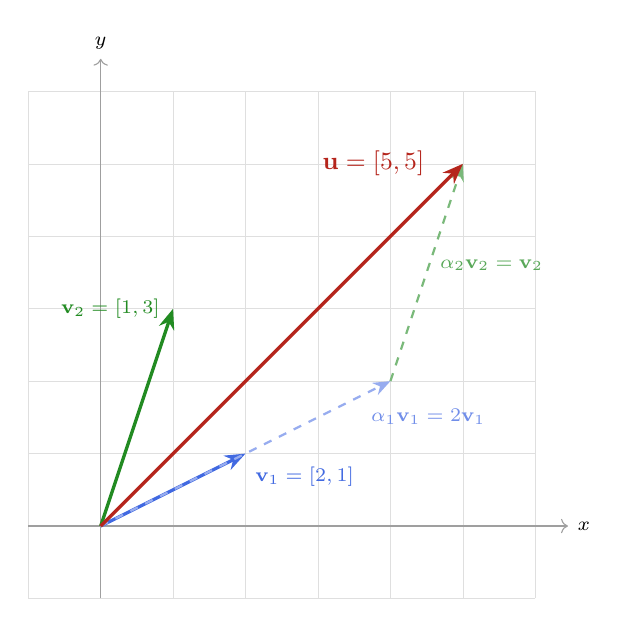
\begin{tikzpicture}[scale=0.92]
  \lattice{-1}{6}{-1}{6}
  \draw[vecarr,RoyalBlue]   (0,0) -- (2,1);
  \draw[vecarr,ForestGreen] (0,0) -- (1,3);
  \draw[thinarr,RoyalBlue!55,dashed]   (0,0) -- (4,2);
  \draw[thinarr,ForestGreen!60,dashed] (4,2) -- (5,5);
  \draw[vecarr,BrickRed]    (0,0) -- (5,5);
  \node[below right,font=\scriptsize,RoyalBlue]   at (2.0,0.95) {$\vc{v}_1=[2,1]$};
  \node[left,font=\scriptsize,ForestGreen]        at (0.95,3.0) {$\vc{v}_2=[1,3]$};
  \node[below right,font=\scriptsize,RoyalBlue!75] at (3.6,1.75) {$\alpha_1\vc{v}_1=2\vc{v}_1$};
  \node[right,font=\scriptsize,ForestGreen!75]    at (4.55,3.6) {$\alpha_2\vc{v}_2=\vc{v}_2$};
  \node[above left,font=\small,BrickRed]          at (4.6,4.7) {$\vc{u}=[5,5]$};
\end{tikzpicture}
\end{center}

\noindent The picture is the same walk as in the vector unit, \S16.5 --- travel
$\alpha_1$ steps along the first basis vector, then $\alpha_2$ along the second,
and arrive at the head of $\vc{u}$ --- but the steps are no longer along the
axes, and that is exactly what makes the arithmetic non-trivial.

\begin{rmk}[What changed, and it is only one thing]
Against the standard basis the same system would have read
$1\alpha_1+0\alpha_2=u_1$ and $0\alpha_1+1\alpha_2=u_2$, and the zeros would
have collapsed it on sight. Here there are no zeros: both unknowns appear in
both equations, so neither can be found without the other, and the equations
have to be handled together. The vector unit predicted this at the end of
\S16.5. Substitution coped with two equations; it is not a method that survives
twenty.
\end{rmk}

%------------------------------------------------------------------------------
\subsection{The same thing one dimension up}
%------------------------------------------------------------------------------
One more, in $\R^{3}$, to have a case with enough room to show the shape of
things. Take
\[
  \vc{v}_1 = [\,1,\,0,\,1\,], \qquad
  \vc{v}_2 = [\,2,\,1,\,0\,], \qquad
  \vc{v}_3 = [\,0,\,1,\,1\,] .
\]
These are independent, and checking it is itself a small system: setting
$\alpha_1\vc{v}_1+\alpha_2\vc{v}_2+\alpha_3\vc{v}_3=\vc{0}$ and reading the
three slots gives $\alpha_1+2\alpha_2=0$, $\alpha_2+\alpha_3=0$ and
$\alpha_1+\alpha_3=0$. The last two give $\alpha_1=\alpha_2=-\alpha_3$, and
substituting into the first gives $-3\alpha_3=0$, so all three are zero. Three
independent vectors in $\R^{3}$, so a basis.

Now suppose the coordinates of some $\vc{u}$ turn out to be
$\alpha_1=1$, $\alpha_2=2$, $\alpha_3=3$. Then
\[
  \vc{u} = 1[\,1,0,1\,] + 2[\,2,1,0\,] + 3[\,0,1,1\,]
         = [\,1,0,1\,] + [\,4,2,0\,] + [\,0,3,3\,]
         = [\,5,\,5,\,4\,] .
\]
Read off the components with the convention of \S1.3 --- $v_{ki}$ is slot $k$ of
$\vc{v}_i$, so $v_{12}=2$ is the first slot of the second vector --- and the
system for the unknown coordinates of $\vc{u}=[5,5,4]$ is
\[
  \begin{aligned}
    1\alpha_1 + 2\alpha_2 + 0\alpha_3 &= 5 ,\\
    0\alpha_1 + 1\alpha_2 + 1\alpha_3 &= 5 ,\\
    1\alpha_1 + 0\alpha_2 + 1\alpha_3 &= 4 ,
  \end{aligned}
\]
whose solution is $\alpha_1=1$, $\alpha_2=2$, $\alpha_3=3$, as constructed. This
is the example \S2 will carry through. Notice already what \S1.3 promised: the
coefficients going \emph{down} the first column are $1,0,1$, which is $\vc{v}_1$;
down the second, $2,1,0$, which is $\vc{v}_2$; down the third, $0,1,1$, which is
$\vc{v}_3$.

%------------------------------------------------------------------------------
\subsection{Where else these come from}
%------------------------------------------------------------------------------
The coordinate problem is how linear systems enter \emph{this} course, and it is
a good entrance because everything about it is already understood: we know a
solution exists, we know it is unique, and we know what it means. It is not the
only entrance. Systems of linear equations arise whenever several linear
constraints must hold at once --- balancing a chemical reaction, fitting a line
through data, computing currents in a circuit, allocating a fixed budget across
competing demands, enforcing conservation at every node of a network.

What all of these share is not their subject matter but their \emph{shape}: a
list of unknowns, and a list of linear equations relating them. That shape is
what the next section names, and naming it is what lets one method serve all of
them.

%==============================================================================
\section{Compressing the notation}
%==============================================================================
The system of \S1.3 is correct and unwieldy. Writing it out costs $n$ lines,
each with $n$ terms, so a system in twenty unknowns fills a page before any work
is done --- and none of that page is doing anything a symbol could not.

Before asking \emph{how} to solve such a system, we spend this section building
notation for it. Four steps, each one small.

%------------------------------------------------------------------------------
\subsection{Step 1: every equation is a dot product}
%------------------------------------------------------------------------------
Look at a single equation of the system --- row $k$:
\[
  \alpha_1 v_{k1} + \alpha_2 v_{k2} + \cdots + \alpha_n v_{kn}
  \;=\; u_k .
\]
The left-hand side is a sum of products of paired-up numbers, which is a
structure we have a name for. Set
\[
  \vc{r}_k = [\,v_{k1},\ v_{k2},\ \dots,\ v_{kn}\,],
  \qquad
  \vc{x}   = [\,\alpha_1,\ \alpha_2,\ \dots,\ \alpha_n\,] ,
\]
and the left-hand side is precisely $\langle\vc{r}_k,\vc{x}\rangle$, the dot
product of the vector unit, \S11.3. So the system is
\[
  \langle\vc{r}_1,\vc{x}\rangle = u_1,
  \qquad
  \langle\vc{r}_2,\vc{x}\rangle = u_2,
  \qquad \dots, \qquad
  \langle\vc{r}_n,\vc{x}\rangle = u_n .
\]
Nothing has been computed and nothing has been assumed. We have only noticed
that an operation we already have describes each line.

\begin{ex}
For the $\R^{3}$ system of \S1.6, the three vectors $\vc{r}_k$ are
$[\,1,2,0\,]$, $[\,0,1,1\,]$ and $[\,1,0,1\,]$, and with $\vc{x}=[\,1,2,3\,]$,
\[
  \begin{aligned}
    \langle[1,2,0],[1,2,3]\rangle &= 1+4+0 = 5, \\
    \langle[0,1,1],[1,2,3]\rangle &= 0+2+3 = 5, \\
    \langle[1,0,1],[1,2,3]\rangle &= 1+0+3 = 4 ,
  \end{aligned}
\]
which are the three right-hand sides $5,5,4$. \hfill$\blacksquare$
\end{ex}

\begin{defn}[Coordinate vector]
The vector $\vc{x}=[\,\alpha_1,\dots,\alpha_n\,]$ holding the unknown
coordinates is the \textbf{coordinate vector} of $\vc{u}$ with respect to
$\bas$.
\end{defn}

\begin{rmk}
Two different vectors of $\R^{n}$ are now in play and it is worth keeping them
apart. The vector $\vc{u}$ is a point of the space. The vector $\vc{x}$ is the
recipe for building it out of $\bas$. They are equal only when $\bas$ is the
standard basis --- which is the content of the vector unit's remark at \S16.4,
that the bracket notation was silently reporting coordinates in one particular
basis all along.
\end{rmk}

%------------------------------------------------------------------------------
\subsection{Step 2: the matrix}
%------------------------------------------------------------------------------
The $n$ vectors $\vc{r}_1,\dots,\vc{r}_n$ carry all the coefficients of the
system, and $\vc{x}$ carries all the unknowns. Stack the $\vc{r}_k$ in order,
one per line, keeping their entries aligned in columns.

\begin{defn}[Matrix]
A \textbf{matrix} is a rectangular array of numbers arranged in rows and
columns. The matrix of the system of \S1.3 is
\[
  \mt{V} \;=\;
  \begin{bmatrix}
    v_{11} & v_{12} & \cdots & v_{1n} \\
    v_{21} & v_{22} & \cdots & v_{2n} \\
    \vdots & \vdots & \ddots & \vdots \\
    v_{n1} & v_{n2} & \cdots & v_{nn}
  \end{bmatrix},
\]
with $n$ rows and $n$ columns. The number $v_{ki}$ in row $k$ and column $i$ is
the \textbf{$(k,i)$ entry} of $\mt{V}$.
\end{defn}

\noindent This is the second object of the course, after the vector, and the
convention of \S1.3 is what makes it painless to write down: the two indices of
$v_{ki}$ are already the two directions of the grid, row first and column
second. Nothing had to be rearranged.

Now the two readings of \S1.3 become geometric facts about the array.

\begin{itemize}[leftmargin=1.4em,itemsep=4pt]
  \item \textbf{Row $k$ of $\mt{V}$ is $\vc{r}_k$}, the coefficients of the
        $k$-th equation. Rows are equations.
  \item \textbf{Column $i$ of $\mt{V}$ is $\vc{v}_i$}, the $i$-th basis vector,
        written downward. Columns are the basis.
\end{itemize}

\noindent So $\mt{V}$ is the basis $\bas$ with its vectors stood up side by side:
\[
  \mt{V} \;=\;
  \left[\;
  \begin{array}{c|c|c|c}
    \rule{0pt}{2.4ex}\vc{v}_1 & \vc{v}_2 & \cdots & \vc{v}_n
  \end{array}
  \;\right] ,
\]
which is worth remembering as the picture of what the matrix \emph{is}, before
it is anything else.

\begin{ex}
The $\R^{3}$ system of \S1.6 has
\[
  \mt{V} =
  \begin{bmatrix}
    1 & 2 & 0 \\
    0 & 1 & 1 \\
    1 & 0 & 1
  \end{bmatrix} .
\]
Its rows $[1,2,0]$, $[0,1,1]$, $[1,0,1]$ are the three equations. Its columns,
read downward, are $[1,0,1]$, $[2,1,0]$, $[0,1,1]$ --- exactly
$\vc{v}_1,\vc{v}_2,\vc{v}_3$. \hfill$\blacksquare$
\end{ex}

%------------------------------------------------------------------------------
\subsection{Step 3: multiplying a matrix by a vector}
%------------------------------------------------------------------------------
We have a matrix holding the coefficients and a vector holding the unknowns, and
\S2.1 said what to do with them: dot each row against $\vc{x}$. Doing that for
every row produces $n$ numbers, which is a vector. So the operation takes a
matrix and a vector and returns a vector, and it deserves a name and a symbol.

\begin{defn}[Matrix--vector product]
Let $\mt{V}$ be an $n\times n$ matrix with rows
$\vc{r}_1,\dots,\vc{r}_n$, and let $\vc{x}\in\R^{n}$. The
\textbf{matrix--vector product} $\mt{V}\vc{x}$ is the vector of $\R^{n}$ whose
$k$-th component is the dot product of row $k$ with $\vc{x}$:
\[
  \mt{V}\vc{x}
  \;=\;
  \begin{bmatrix}
    \langle\vc{r}_1,\vc{x}\rangle \\
    \langle\vc{r}_2,\vc{x}\rangle \\
    \vdots \\
    \langle\vc{r}_n,\vc{x}\rangle
  \end{bmatrix}
  \;=\;
  \begin{bmatrix}
    \displaystyle\sum_{i=1}^{n} v_{1i}\,\alpha_i \\[4pt]
    \displaystyle\sum_{i=1}^{n} v_{2i}\,\alpha_i \\
    \vdots \\
    \displaystyle\sum_{i=1}^{n} v_{ni}\,\alpha_i
  \end{bmatrix} .
\]
\end{defn}

\noindent In words, and this is the sentence to memorise: \emph{to multiply a
matrix by a vector, take the dot product of each row of the matrix with that
vector.} The row supplies one component of the answer, and there are as many
components as rows.

\begin{center}
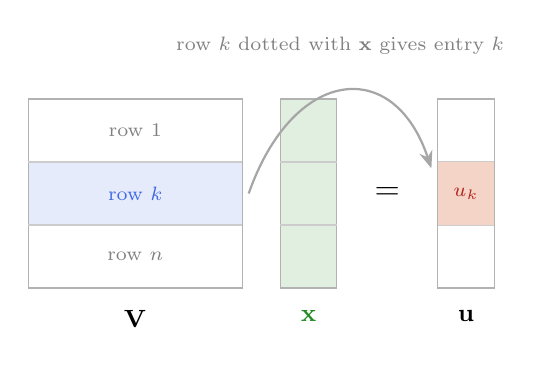
\begin{tikzpicture}[x=0.8cm,y=0.8cm]
  % --- V: three row bands, no internal column rules; rows are the unit here
  \fill[RoyalBlue!13] (0,1) rectangle (3.4,2);
  \draw[gray!60] (0,0) rectangle (3.4,3);
  \foreach \y in {1,2} { \draw[gray!40] (0,\y) -- (3.4,\y); }
  \node[font=\scriptsize,gray]      at (1.7,2.5) {row $1$};
  \node[font=\scriptsize,RoyalBlue] at (1.7,1.5) {row $k$};
  \node[font=\scriptsize,gray]      at (1.7,0.5) {row $n$};
  \node[below,font=\small] at (1.7,-0.2) {$\mt{V}$};
  % --- x: one column, n cells
  \fill[ForestGreen!14] (4.0,0) rectangle (4.9,3);
  \draw[gray!60] (4.0,0) rectangle (4.9,3);
  \foreach \y in {1,2} { \draw[gray!40] (4.0,\y) -- (4.9,\y); }
  \node[below,font=\small,ForestGreen] at (4.45,-0.2) {$\vc{x}$};
  \node[font=\large] at (5.7,1.5) {$=$};
  % --- u: one column, entry k highlighted
  \draw[gray!60] (6.5,0) rectangle (7.4,3);
  \foreach \y in {1,2} { \draw[gray!40] (6.5,\y) -- (7.4,\y); }
  \fill[BrickRed!15] (6.5,1) rectangle (7.4,2);
  \node[font=\scriptsize,BrickRed] at (6.95,1.5) {$u_k$};
  \node[below,font=\small] at (6.95,-0.2) {$\vc{u}$};
  % --- the one operation the picture is about
  \draw[thinarr,gray!70]
        (3.5,1.5) .. controls (4.2,3.5) and (5.8,3.7) .. (6.4,1.9);
  \node[font=\scriptsize,gray] at (4.95,3.85)
       {row $k$ dotted with $\vc{x}$ gives entry $k$};
\end{tikzpicture}
\end{center}

\begin{warn}[Rows, columns, and the bracket notation]
The vector unit wrote vectors horizontally, $\vc{v}=[\,v_1,\dots,v_n\,]$, and
the display above writes $\vc{x}$ and $\mt{V}\vc{x}$ vertically. Nothing has
changed about the vectors. The bracket notation never claimed a shape --- it
listed $n$ numbers in order, which is all a vector in $\R^{n}$ is --- and
$[\,1,2,3\,]$ and its column spelling denote the same element of $\R^{3}$.

The reason for switching is that $\mt{V}\vc{x}$ dots $\vc{x}$ against each
\emph{row}, so drawing $\vc{x}$ as a column puts each of its entries directly
beneath the column of $\mt{V}$ it multiplies, and the arithmetic can be read off
the page. Horizontal brackets stay in use for prose, where they take less room.
When the distinction between a row and a column starts to carry mathematical
weight, we will say so; here it is typography.
\end{warn}

\begin{ex}
With $\mt{V}$ from \S2.2 and $\vc{x}=[\,1,\,2,\,3\,]$:
\[
  \begin{bmatrix}
    1 & 2 & 0 \\
    0 & 1 & 1 \\
    1 & 0 & 1
  \end{bmatrix}
  \begin{bmatrix} 1 \\ 2 \\ 3 \end{bmatrix}
  =
  \begin{bmatrix}
    1(1) + 2(2) + 0(3) \\
    0(1) + 1(2) + 1(3) \\
    1(1) + 0(2) + 1(3)
  \end{bmatrix}
  =
  \begin{bmatrix} 5 \\ 5 \\ 4 \end{bmatrix} .
\]
Three dot products, three components. \hfill$\blacksquare$
\end{ex}

\begin{rmk}[A shape rule, for later]
Row $k$ has $n$ entries and $\vc{x}$ has $n$ entries, and a dot product is
defined only when both vectors have the same dimension (the vector unit,
\S11.3). So $\mt{V}\vc{x}$ makes sense only when the number of \emph{columns} of
$\mt{V}$ matches the number of entries of $\vc{x}$. Every matrix in this part is
$n\times n$ and the condition is automatic, but it is the rule that will govern
all matrix multiplication later, and it comes from nowhere more exotic than the
dot product needing two vectors of equal length.
\end{rmk}

%------------------------------------------------------------------------------
\subsection{Step 4: \texorpdfstring{$\mt{V}\vc{x}=\vc{u}$}{Vx = u}}
%------------------------------------------------------------------------------
Now put the three pieces together. By \S2.3, the $k$-th component of
$\mt{V}\vc{x}$ is $\langle\vc{r}_k,\vc{x}\rangle$. By \S2.1, the $k$-th equation
of the system says that this equals $u_k$. Two vectors are equal exactly when
all their components agree. So the entire system --- all $n$ equations, all $n$
unknowns --- is the single statement
\[
  \boxed{\;\mt{V}\vc{x} = \vc{u}\;}
\]

That is the compression. The $\R^{3}$ example of \S1.6, which took three lines
and nine coefficients to state, is
\[
  \begin{bmatrix}
    1 & 2 & 0 \\
    0 & 1 & 1 \\
    1 & 0 & 1
  \end{bmatrix}
  \begin{bmatrix} \alpha_1 \\ \alpha_2 \\ \alpha_3 \end{bmatrix}
  =
  \begin{bmatrix} 5 \\ 5 \\ 4 \end{bmatrix} ,
\]
and in $\R^{20}$ it would still be $\mt{V}\vc{x}=\vc{u}$.

\begin{center}
\renewcommand{\arraystretch}{1.35}
\begin{tabular}{@{}l l l@{}}
\toprule
\textbf{Symbol} & \textbf{What it is} & \textbf{Known?} \\
\midrule
$\mt{V}$   & the $n\times n$ matrix whose columns are the basis vectors & known \\
$\vc{x}$   & the coordinate vector $[\,\alpha_1,\dots,\alpha_n\,]$      & \textbf{unknown} \\
$\vc{u}$   & the vector whose coordinates we want                       & known \\
\bottomrule
\end{tabular}
\end{center}

\noindent Compare the shape of $\mt{V}\vc{x}=\vc{u}$ with the scalar equation
$ax=b$, whose solution is $x=b/a$ whenever $a\neq0$. The resemblance is not
accidental and it is not yet a method: we have no division of vectors, and no
meaning for $\mt{V}^{-1}$. But the resemblance is the reason the notation is
worth having. It makes a question of $n$ equations look like a question about
one object, and questions about one object are the kind we know how to ask.

\begin{rmk}[What was actually gained]
Three things, and only the first is about saving ink.

\emph{Brevity.} One symbol for $n^{2}$ coefficients.

\emph{Uniformity.} The coordinate problem, a circuit, a least-squares fit and a
network flow all reduce to $\mt{V}\vc{x}=\vc{u}$ with different $\mt{V}$. A
method for the equation is a method for all of them at once.

\emph{A new object.} $\mt{V}$ was introduced as bookkeeping, but it will not
stay bookkeeping. Matrices add, multiply, and have their own arithmetic; a
matrix will turn out to \emph{act} on vectors rather than merely tabulate
numbers, and $\mt{V}\vc{x}$ will be read as a function applied to $\vc{x}$. That
reading is where most of the rest of this course lives.
\end{rmk}

%------------------------------------------------------------------------------
\subsection{The same equation, read by columns}
%------------------------------------------------------------------------------
The definition in \S2.3 built $\mt{V}\vc{x}$ out of rows. There is a second way
to read the same product, and it closes the loop back to \S1.1.

Take the $\R^{3}$ computation again, and instead of collecting the arithmetic
into three dot products, group it by which column of $\mt{V}$ each term came
from:
\[
  \begin{bmatrix}
    1(1) + 2(2) + 0(3) \\
    0(1) + 1(2) + 1(3) \\
    1(1) + 0(2) + 1(3)
  \end{bmatrix}
  =
  1\begin{bmatrix} 1 \\ 0 \\ 1 \end{bmatrix}
  + 2\begin{bmatrix} 2 \\ 1 \\ 0 \end{bmatrix}
  + 3\begin{bmatrix} 0 \\ 1 \\ 1 \end{bmatrix} .
\]
The left side is grouped by row, the right side by column, and both are the same
nine products added in a different order. But the right-hand side is
$\alpha_1\vc{v}_1+\alpha_2\vc{v}_2+\alpha_3\vc{v}_3$ --- a linear combination of
the basis vectors, with the entries of $\vc{x}$ as the weights.

\begin{thm}[The two readings of a matrix--vector product]
Let $\mt{V}$ have columns $\vc{v}_1,\dots,\vc{v}_n$ and let
$\vc{x}=[\,\alpha_1,\dots,\alpha_n\,]$. Then
\[
  \mt{V}\vc{x}
  \;=\;
  \underbrace{\bigl[\,\langle\vc{r}_1,\vc{x}\rangle,\ \dots,\
                      \langle\vc{r}_n,\vc{x}\rangle\,\bigr]}_{\text{by rows}}
  \;=\;
  \underbrace{\alpha_1\vc{v}_1 + \alpha_2\vc{v}_2 + \cdots
              + \alpha_n\vc{v}_n}_{\text{by columns}} .
\]
\end{thm}

\begin{proof}
Compare slot $k$ of each side. On the left it is
$\langle\vc{r}_k,\vc{x}\rangle=\sum_{i=1}^{n}v_{ki}\alpha_i$, by \S2.3. On the
right, slot $k$ of $\alpha_i\vc{v}_i$ is $\alpha_i v_{ki}$, since scaling acts
componentwise, and adding the $n$ vectors adds their $k$-th slots, giving
$\sum_{i=1}^{n}\alpha_i v_{ki}$. The two sums have the same terms.
\end{proof}

\noindent So $\mt{V}\vc{x}=\vc{u}$ says, in the column reading,
\[
  \alpha_1\vc{v}_1 + \alpha_2\vc{v}_2 + \cdots + \alpha_n\vc{v}_n = \vc{u} ,
\]
which is the boxed equation of \S1.1 --- the one we started from. We have gone
around a full circle and arrived back where we began, in new notation.

\begin{rmk}[Why the circle was worth walking]
Nothing was proved on the trip; the two ends are the same statement. What
changed is that the statement now has a \emph{form}, and the form is what can be
worked on. ``Find weights that combine these vectors into $\vc{u}$'' is a
description. ``Solve $\mt{V}\vc{x}=\vc{u}$'' is a problem with an object in it.

Keep both readings. The row reading is how you \emph{compute} a matrix--vector
product, and it is what an algorithm implements. The column reading is how you
\emph{understand} one: $\mt{V}\vc{x}$ is a linear combination of the columns of
$\mt{V}$. Most of the structural theorems ahead --- when a system has a
solution, how many, what the columns of a matrix span --- are consequences of the
column reading.
\end{rmk}

\begin{warn}[$\mt{V}$ is not a list of the basis vectors]
Writing $\mt{V}$ as its columns is a picture, not an identification. A basis is a
\emph{set} --- $\bas=\{\vc{v}_1,\dots,\vc{v}_n\}$, unordered, with no repeats. A
matrix is an \emph{array}, in which order matters and entries may repeat.
Swapping two columns of $\mt{V}$ gives a different matrix but the same basis,
with the coordinates permuted to match. So $\mt{V}$ records the basis
\emph{together with} a choice of ordering for it, which the set $\bas$ alone does
not supply.
\end{warn}

%------------------------------------------------------------------------------
\subsection{Practice}
%------------------------------------------------------------------------------
\begin{enumerate}[label=\textbf{P\arabic*.},leftmargin=2.6em,itemsep=5pt]
  \item Let $\vc{v}_1=[\,3,\,1\,]$ and $\vc{v}_2=[\,1,\,2\,]$, and let
        $\vc{u}=[\,7,\,4\,]$. Write the system for the coordinates of $\vc{u}$,
        solve it, and check your answer in the original vector equation.
  \item Write the matrix $\mt{V}$ for the basis in P1, and verify that
        $\mt{V}\vc{x}=\vc{u}$ for the $\vc{x}$ you found.
  \item Compute
        $\begin{bmatrix} 2 & -1 & 0 \\ 1 & 1 & 3 \\ 0 & 4 & -2 \end{bmatrix}
         \begin{bmatrix} 1 \\ 2 \\ -1 \end{bmatrix}$
        twice: once by the row reading, once by the column reading. The answers
        must agree.
  \item Let $\bas=\{\vc{e}_1,\dots,\vc{e}_n\}$ be the standard basis of
        $\R^{n}$. Write down $\mt{V}$, and use \S2.5 to say in one sentence why
        the system $\mt{V}\vc{x}=\vc{u}$ has solution $\vc{x}=\vc{u}$.
  \item Suppose $\vc{v}_1=[\,1,\,2\,]$ and $\vc{v}_2=[\,2,\,4\,]$. Show that the
        system for the coordinates of $\vc{u}=[\,3,\,1\,]$ has no solution, and
        say which hypothesis of \S1.1 fails.
\end{enumerate}

\subsubsection*{Answer key}

\noindent\textbf{P1.} The system is $3\alpha_1+\alpha_2=7$ and
$\alpha_1+2\alpha_2=4$. From the first, $\alpha_2=7-3\alpha_1$; substituting,
$\alpha_1+14-6\alpha_1=4$, so $-5\alpha_1=-10$ and $\alpha_1=2$, then
$\alpha_2=1$. Check: $2[\,3,1\,]+1[\,1,2\,]=[\,6,2\,]+[\,1,2\,]=[\,7,4\,]$.
\checkmark

\smallskip
\noindent\textbf{P2.} The columns of $\mt{V}$ are the basis vectors, so
$\mt{V}=\begin{bmatrix} 3 & 1 \\ 1 & 2\end{bmatrix}$ and
$\vc{x}=[\,2,\,1\,]$. Row $1$: $3(2)+1(1)=7$. Row $2$: $1(2)+2(1)=4$. So
$\mt{V}\vc{x}=[\,7,\,4\,]=\vc{u}$. \checkmark

\smallskip
\noindent\textbf{P3.} By rows: $2(1)-1(2)+0(-1)=0$; $1(1)+1(2)+3(-1)=0$;
$0(1)+4(2)-2(-1)=10$. So the product is $[\,0,\,0,\,10\,]$. By columns:
\[
  1\begin{bmatrix}2\\1\\0\end{bmatrix}
  + 2\begin{bmatrix}-1\\1\\4\end{bmatrix}
  + (-1)\begin{bmatrix}0\\3\\-2\end{bmatrix}
  = \begin{bmatrix}2\\1\\0\end{bmatrix}
  + \begin{bmatrix}-2\\2\\8\end{bmatrix}
  + \begin{bmatrix}0\\-3\\2\end{bmatrix}
  = \begin{bmatrix}0\\0\\10\end{bmatrix} . \quad\checkmark
\]

\smallskip
\noindent\textbf{P4.} The columns are $\vc{e}_1,\dots,\vc{e}_n$, so $\mt{V}$ has
$1$s down the diagonal and $0$s elsewhere. By the column reading,
$\mt{V}\vc{x}=\alpha_1\vc{e}_1+\cdots+\alpha_n\vc{e}_n=[\,\alpha_1,\dots,\alpha_n\,]=\vc{x}$,
so the equation reads $\vc{x}=\vc{u}$ directly. This is the vector unit's
observation at \S24.1 that coordinates against the standard basis are the
components themselves, now visible as a property of one particular matrix.

\smallskip
\noindent\textbf{P5.} The system is $\alpha_1+2\alpha_2=3$ and
$2\alpha_1+4\alpha_2=1$. The second equation is twice the left-hand side of the
first, so it demands $2(3)=1$, which is false; no pair
$(\alpha_1,\alpha_2)$ satisfies both. The hypothesis that fails is
\emph{independence}: $\vc{v}_2=2\vc{v}_1$, so $\bas$ is linearly dependent (the
vector unit, \S18.4), hence not a basis, and its span is a line rather than
$\R^{2}$ --- a line that does not contain $[\,3,\,1\,]$. With the basis
hypothesis gone, so is the guarantee of \S1.1 that a solution exists at all.

\lookahead We can now state the problem in one line but not yet solve it. Before
a method for solving it is worth writing down, the object it operates on
deserves a proper definition. So far $\mt{V}$ has been \emph{a} matrix --- the
one that happened to fall out of one particular problem, with the basis vectors
down its columns. The rest of this document steps back from that problem
entirely and asks what a matrix is in general, what shapes they come in, and
what you are allowed to do to them.

%==============================================================================
\section{What a matrix is}
%==============================================================================

%------------------------------------------------------------------------------
\subsection{The definition}
%------------------------------------------------------------------------------
\begin{defn}[Matrix]
Let $m,n\in\N$. An \textbf{$m\times n$ matrix} (read ``$m$ by $n$'') is a
two-dimensional grid of numbers arranged in $m$ rows and $n$ columns. The
numbers $m$ and $n$ are its \textbf{dimensions}. Each number in the grid is an
\textbf{entry}, and the entry in row $i$ and column $j$ is written $a_{ij}$.
\end{defn}

\noindent Written out, a matrix $\mt{A}$ is
\[
  \mt{A} \;=\;
  \begin{bmatrix}
    a_{11} & a_{12} & a_{13} & \cdots & a_{1n}\\
    a_{21} & a_{22} & a_{23} & \cdots & a_{2n}\\
    a_{31} & a_{32} & a_{33} & \cdots & a_{3n}\\
    \vdots & \vdots & \vdots & \ddots & \vdots\\
    a_{m1} & a_{m2} & a_{m3} & \cdots & a_{mn}
  \end{bmatrix} .
\]
Read an index in two steps: $a_{ij}$ sits in \emph{row $i$}, then \emph{column
$j$}. Row first, column second --- always. So $a_{23}$ is in the second row and
third column, and $a_{32}$ is in the third row and second column; these are
different positions and in general different numbers. Every entry has exactly
one such address, and every address names exactly one entry, which is what makes
the grid an unambiguous way of storing $mn$ numbers.

\lookback This is the same convention \S1.3 fixed for the basis vectors, where
$v_{ki}$ meant component $k$ of vector $i$ and sat in row $k$, column $i$ of
$\mt{V}$. Nothing has changed; it is now stated for a matrix in general rather
than for that one matrix.

\begin{warn}[$2\times3$ is not $3\times2$]
The dimensions are an \emph{ordered} pair and the order is rows-then-columns. A
$2\times3$ matrix is short and wide --- two rows, three columns. A $3\times2$
matrix is tall and narrow. Reversing them describes a different object, and in
\S8 it will be the difference between a product that is defined and one that is
not.
\end{warn}

%------------------------------------------------------------------------------
\subsection{Where the entries come from}
%------------------------------------------------------------------------------
The definition said ``numbers'' without saying which. The entries are drawn from
some agreed numerical set: the real numbers $\R$, the integers $\Z$, the complex
numbers $\C$, and others besides. A set of numbers in which you can add,
subtract, multiply, and divide, and have the familiar rules of arithmetic hold,
is called a \textbf{field}. Both $\R$ and $\C$ are fields. The formal definition
is beyond this course; we need the word only to say where the entries live.

\medskip
\noindent\textbf{For the remainder of this document, every matrix entry is a
real number.}

Once the entry set is fixed, we can name the collection of all matrices of a
given shape.

\begin{defn}[The set $\R^{m\times n}$]
$\R^{m\times n}$ denotes the set of all $m\times n$ matrices whose entries are
real numbers. Writing $\mt{A}\in\R^{m\times n}$ says that $\mt{A}$ is an
$m\times n$ matrix holding $mn$ real scalars.
\end{defn}

\noindent The notation is deliberately parallel to $\R^{n}$ from the vector
unit's \S24.1: there, $n$ real numbers in a list; here, $m\times n$ real numbers
in a grid. In both cases the superscript records the shape.

\begin{warn}[$\R^{m\times n}$ is not a field]
$\R$ is a field. $\R^{m\times n}$ is not, and the notation is not claiming it
is --- it is only the \emph{name of a set}, exactly as $\R^{n}$ was. The
difference is easy to state even now: in a field you can divide by any nonzero
element, and there is no general way to divide by a matrix. We will see in \S8
that matrices fail an even more basic test, since $\mt{A}\mt{B}$ and
$\mt{B}\mt{A}$ need not be equal.
\end{warn}

\noindent As \S2.2 already noted, capital letters conventionally denote
matrices, lower case denotes vectors and scalars. That convention is why
$\mt{A}\in\R^{m\times n}$ can be read at a glance.

%------------------------------------------------------------------------------
\subsection{Examples}
%------------------------------------------------------------------------------
\begin{ex}
Three matrices from three different sets.
\[
  \mt{A}=\begin{bmatrix}1&0\\0&1\end{bmatrix}\in\R^{2\times2},
  \qquad
  \mt{B}=\begin{bmatrix}2&3\\4&5\\6&7\end{bmatrix}\in\R^{3\times2},
  \qquad
  \mt{D}=\begin{bmatrix}
    \pi & e & \pi & e\\[2pt]
    \tfrac12 & \tfrac13 & \tfrac14 & \tfrac15
  \end{bmatrix}\in\R^{2\times4} .
\]
Reading entries out of them:
\[
  a_{12}=0,\qquad
  b_{32}=7,\qquad
  b_{21}=4,\qquad
  d_{14}=e,\qquad
  d_{23}=\tfrac14 .
\]
Check $b_{32}$ against the grid: third row, second column --- the row is
$[\,6,\ 7\,]$ and its second entry is $7$. And note that $\mt{B}$ has no entry
$b_{23}$: it has only two columns, so the address does not exist.
\end{ex}

\begin{rmk}
$\mt{A}$ above is a matrix you have already met. Its columns are $\vc{e}_1$ and
$\vc{e}_2$, the standard basis of $\R^{2}$, so it is the matrix that appeared in
P4 of \S2.6 --- the one for which $\mt{V}\vc{x}=\vc{x}$. It gets a name in
\S4.3.
\end{rmk}

%------------------------------------------------------------------------------
\subsection{A vector is a matrix}
%------------------------------------------------------------------------------
Nothing in the definition forbids $m=1$ or $n=1$. Those two cases should look
familiar.

If $\mt{A}\in\R^{1\times n}$ then $\mt{A}$ has one row and $n$ columns:
\[
  \mt{A}=\begin{bmatrix}a_{11}&a_{12}&a_{13}&\cdots&a_{1n}\end{bmatrix} ,
\]
which is a list of $n$ numbers --- a vector. Laid out this way it is called a
\textbf{row vector}. If instead $\mt{A}\in\R^{m\times1}$, there is one column
and $m$ rows:
\[
  \mt{A}=\begin{bmatrix}a_{11}\\a_{21}\\a_{31}\\\vdots\\a_{m1}\end{bmatrix} ,
\]
a \textbf{column vector}. Both hold the same kind of data as a vector in the
sense of the vector unit; they differ only in whether that data is written
across or down.

\lookback \S2.3 flagged this and set it aside: the bracket notation
$[\,v_1,\dots,v_n\,]$ never asserted a shape, and the row and column spellings
denote the same vector. Now that matrices are defined in general, the two
spellings are genuinely different \emph{matrices} --- one is $1\times n$, the
other $n\times1$ --- even though they carry identical numbers. \S6.3 gives the
operation that converts between them.

%------------------------------------------------------------------------------
\subsection{Rows and columns}
%------------------------------------------------------------------------------
Because a single row is a row vector and a single column is a column vector,
an $m\times n$ matrix admits two readings, and both are useful.

\begin{center}
\renewcommand{\arraystretch}{1.3}
\begin{tabular}{@{}l p{10.4cm}@{}}
\toprule
\textbf{Reading} & \textbf{What the matrix is} \\
\midrule
\textbf{By rows}    & A stack of $m$ row vectors, each with $n$ components,
                      laid one on top of the next. \\
\textbf{By columns} & A shelf of $n$ column vectors, each with $m$ components,
                      standing side by side. \\
\bottomrule
\end{tabular}
\end{center}

\noindent For $\mt{B}\in\R^{3\times2}$ above, the row reading gives three
vectors in $\R^{2}$ --- $[\,2,3\,]$, $[\,4,5\,]$, $[\,6,7\,]$ --- and the column
reading gives two vectors in $\R^{3}$ --- $[\,2,4,6\,]$ and $[\,3,5,7\,]$.
Same six numbers, grouped two different ways.

\lookback Both readings have already done work. \S2.4 computed
$\mt{V}\vc{x}$ by rows, as $n$ dot products; \S2.5 computed the same product by
columns, as one linear combination of the basis vectors. That the two agree was
the point of \S2.5, and it is a fact about every matrix, not just $\mt{V}$.

%==============================================================================
\section{Shapes and patterns}
%==============================================================================
Matrices are classified first by shape --- the relationship between $m$ and $n$
--- and then by where their nonzero entries sit. The vocabulary below is used
constantly, because knowing that a matrix has a particular pattern usually means
there is a faster way to work with it.

%------------------------------------------------------------------------------
\subsection{Square and rectangular}
%------------------------------------------------------------------------------
\begin{defn}
A matrix $\mt{A}\in\R^{n\times n}$, with as many rows as columns, is
\textbf{square}. A matrix $\mt{A}\in\R^{m\times n}$ with $m\neq n$ is
\textbf{rectangular}.
\end{defn}

\noindent The distinction matters more than it looks. A square matrix maps
$\R^{n}$ to itself and can be multiplied by itself; a rectangular one cannot.
The coefficient matrix $\mt{V}$ of \S2.2 was square precisely because a basis of
$\R^{n}$ has exactly $n$ vectors, each with $n$ components --- and that squareness
is what made ``$n$ equations in $n$ unknowns'' possible.

\[
  \underbrace{\begin{bmatrix}1&5\\-2&3\end{bmatrix}}_{2\times2,\ \text{square}}
  \qquad
  \underbrace{\begin{bmatrix}2&3\\4&5\\6&7\end{bmatrix}}_{3\times2,\ \text{rectangular}}
  \qquad
  \underbrace{\begin{bmatrix}1&0&4&2\\7&1&0&3\end{bmatrix}}_{2\times4,\ \text{rectangular}}
\]

\begin{rmk}[The $1\times1$ case]
A $1\times1$ matrix $[\,a_{11}\,]$ is technically square, but it holds a single
number and behaves like one. It is normally read as the scalar $a_{11}$ rather
than treated as a matrix at all. This is not a quibble --- \S7.1 depends on it.
\end{rmk}

%------------------------------------------------------------------------------
\subsection{The diagonal}
%------------------------------------------------------------------------------
The entries $a_{11},a_{22},a_{33},\dots$ --- those with equal row and column
index --- form the \textbf{main diagonal}, running from the top-left corner
downward. Everything else is \emph{off-diagonal}.

\begin{defn}
A square matrix is \textbf{diagonal} if every off-diagonal entry is zero:
$a_{ij}=0$ whenever $i\neq j$.
\end{defn}

\[
  \begin{bmatrix}3&0&0\\0&-1&0\\0&0&5\end{bmatrix}
  \quad\text{is diagonal, and is written }\ \diagop(3,-1,5).
\]

\noindent A diagonal matrix is described completely by $n$ numbers rather than
$n^{2}$, and almost everything one does with matrices becomes easy when they are
diagonal --- a recurring theme later in the course.

%------------------------------------------------------------------------------
\subsection{The identity}
%------------------------------------------------------------------------------
\begin{defn}
The \textbf{identity matrix} $\mt{I}_n\in\R^{n\times n}$ is the diagonal matrix
whose diagonal entries are all $1$:
\[
  (\mt{I}_n)_{ij}=\begin{cases}1&i=j\\0&i\neq j\end{cases}
  \qquad
  \mt{I}_3=\begin{bmatrix}1&0&0\\0&1&0\\0&0&1\end{bmatrix} .
\]
The subscript is dropped when the size is clear.
\end{defn}

\noindent Its columns are exactly $\vc{e}_1,\dots,\vc{e}_n$, so $\mt{I}$ is the
matrix of the standard basis --- which is why P4 of \S2.6 found
$\mt{I}\vc{x}=\vc{x}$. \S8.4 states the corresponding fact for matrices.

%------------------------------------------------------------------------------
\subsection{Triangular}
%------------------------------------------------------------------------------
\begin{defn}
A square matrix is \textbf{upper triangular} if every entry below the main
diagonal is zero ($a_{ij}=0$ for $i>j$), and \textbf{lower triangular} if every
entry above it is zero ($a_{ij}=0$ for $i<j$).
\end{defn}

\[
  \underbrace{\begin{bmatrix}1&2&3\\0&4&5\\0&0&6\end{bmatrix}}_{\text{upper triangular}}
  \qquad\qquad
  \underbrace{\begin{bmatrix}1&0&0\\2&3&0\\4&5&6\end{bmatrix}}_{\text{lower triangular}}
\]

\noindent A matrix that is both upper and lower triangular has zeros above
\emph{and} below the diagonal --- that is, it is diagonal.

\lookahead Triangular matrices are not a curiosity. A triangular system of
equations can be solved by reading off one unknown at a time and substituting
backwards, with no simultaneous juggling at all. Turning a general system into a
triangular one is exactly what the solution method announced at the end of this
document does.

%------------------------------------------------------------------------------
\subsection{Banded}
%------------------------------------------------------------------------------
\begin{defn}
A matrix is \textbf{banded} if its nonzero entries are confined to a band of
diagonals around the main diagonal --- that is, $a_{ij}=0$ whenever $|i-j|$
exceeds some small fixed width.
\end{defn}

\noindent The narrowest interesting case is \textbf{tridiagonal}: nonzeros only
on the main diagonal and the two diagonals adjacent to it, so $a_{ij}=0$ when
$|i-j|>1$.
\[
  \begin{bmatrix}
     2&-1& 0& 0\\
    -1& 2&-1& 0\\
     0&-1& 2&-1\\
     0& 0&-1& 2
  \end{bmatrix}
\]
Diagonal matrices are the case $|i-j|>0$, so ``diagonal'' is the narrowest band
of all. Bands of width $1$ and $2$ turn up constantly in problems where each
quantity interacts only with its immediate neighbours.

%------------------------------------------------------------------------------
\subsection{Sparse and dense}
%------------------------------------------------------------------------------
\begin{defn}
A matrix is \textbf{sparse} if most of its entries are zero, and \textbf{dense}
if most are nonzero.
\end{defn}

\noindent Unlike the previous definitions this one is deliberately informal ---
there is no fixed fraction at which a matrix becomes sparse. The working test is
practical: a matrix is sparse if it pays to store and process only the nonzero
entries and ignore the rest.
\[
  \underbrace{\begin{bmatrix}
    0&0&4&0&0\\
    0&0&0&0&0\\
    7&0&0&0&1\\
    0&0&0&0&0\\
    0&2&0&0&0
  \end{bmatrix}}_{\text{sparse: }5\text{ nonzeros out of }25}
  \qquad\qquad
  \underbrace{\begin{bmatrix}
    3&1&4\\1&5&9\\2&6&5
  \end{bmatrix}}_{\text{dense: no zeros at all}}
\]
Diagonal, triangular and banded matrices are all sparse, and their sparsity has
a \emph{known shape} --- you can say in advance which entries are zero. General
sparse matrices need not have any pattern; they are simply mostly empty. Real
problems produce enormous sparse matrices routinely: a matrix with a million
rows and only a handful of nonzeros per row is entirely ordinary, and storing it
as a full grid would be hopeless.

%------------------------------------------------------------------------------
\subsection{Summary}
%------------------------------------------------------------------------------
\begin{center}
\renewcommand{\arraystretch}{1.35}
\begin{tabular}{@{}l l p{6.5cm}@{}}
\toprule
\textbf{Name} & \textbf{Condition} & \textbf{In words} \\
\midrule
Square      & $m=n$                       & as many rows as columns \\
Rectangular & $m\neq n$                   & more of one than the other \\
Diagonal    & $a_{ij}=0$ for $i\neq j$    & only the main diagonal survives \\
Identity    & diagonal, all $a_{ii}=1$    & the diagonal is all ones \\
Upper triangular & $a_{ij}=0$ for $i>j$   & nothing below the diagonal \\
Lower triangular & $a_{ij}=0$ for $i<j$   & nothing above the diagonal \\
Banded      & $a_{ij}=0$ for $|i-j|>w$    & confined near the diagonal \\
Sparse      & mostly zeros                & few enough nonzeros to exploit \\
Dense       & mostly nonzeros             & no structure to exploit \\
\bottomrule
\end{tabular}
\end{center}

%==============================================================================
\section{Adding matrices}
%==============================================================================

%------------------------------------------------------------------------------
\subsection{The definition}
%------------------------------------------------------------------------------
\begin{defn}[Matrix addition]
Let $\mt{A},\mt{B}\in\R^{m\times n}$ --- \emph{the same shape}. Their
\textbf{sum} $\mt{A}+\mt{B}\in\R^{m\times n}$ is formed entrywise:
\[
  (\mt{A}+\mt{B})_{ij} \;=\; a_{ij}+b_{ij}
  \qquad\text{for every } i,j .
\]
Subtraction is defined the same way, $(\mt{A}-\mt{B})_{ij}=a_{ij}-b_{ij}$.
\end{defn}

\noindent Each entry minds its own business: the entry in row $i$, column $j$ of
the answer depends only on the entries in that same position of the two inputs.
Nothing mixes across positions.

\begin{warn}[The shapes must match]
$\mt{A}+\mt{B}$ is \emph{undefined} unless $\mt{A}$ and $\mt{B}$ have the same
number of rows \emph{and} the same number of columns. There is no way to add a
$3\times2$ to a $2\times2$: some entries would have no partner. This is the same
restriction the vector unit placed on adding vectors (\S7.1) --- you cannot add
a vector in $\R^{2}$ to one in $\R^{3}$ --- and for the same reason.
\end{warn}

%------------------------------------------------------------------------------
\subsection{Examples}
%------------------------------------------------------------------------------
\begin{ex}
Three sums and one non-sum.
\[
  \begin{bmatrix}1&2\\3&4\end{bmatrix}
  +\begin{bmatrix}5&6\\7&8\end{bmatrix}
  =\begin{bmatrix}1{+}5&2{+}6\\3{+}7&4{+}8\end{bmatrix}
  =\begin{bmatrix}6&8\\10&12\end{bmatrix}
\]
\[
  \begin{bmatrix}5&6\\7&8\end{bmatrix}
  -\begin{bmatrix}1&2\\3&4\end{bmatrix}
  =\begin{bmatrix}4&4\\4&4\end{bmatrix},
  \qquad
  \begin{bmatrix}2&3\\4&5\\6&7\end{bmatrix}
  +\begin{bmatrix}0&1\\1&0\\-6&-7\end{bmatrix}
  =\begin{bmatrix}2&4\\5&5\\0&0\end{bmatrix}
\]
\[
  \begin{bmatrix}2&3\\4&5\\6&7\end{bmatrix}
  +\begin{bmatrix}1&0\\0&1\end{bmatrix}
  \quad\text{is undefined: } 3\times2 \text{ against } 2\times2 .
\]
\end{ex}

%------------------------------------------------------------------------------
\subsection{Scaling a matrix}
%------------------------------------------------------------------------------
One more operation is needed before the laws can be stated. For a scalar
$c\in\R$ and $\mt{A}\in\R^{m\times n}$, the \textbf{scalar multiple} $c\mt{A}$
multiplies every entry by $c$:
\[
  (c\mt{A})_{ij}=c\,a_{ij},
  \qquad\text{for example}\qquad
  3\begin{bmatrix}1&-2\\0&4\end{bmatrix}
  =\begin{bmatrix}3&-6\\0&12\end{bmatrix} .
\]
In particular $-\mt{A}=(-1)\mt{A}$ negates every entry, and
$\mt{A}-\mt{B}=\mt{A}+(-\mt{B})$ --- subtraction is addition of the negative,
exactly as it was for vectors (\S7.3 of the vector unit).

The \textbf{zero matrix} $\mt{0}\in\R^{m\times n}$ has every entry equal to $0$.

%------------------------------------------------------------------------------
\subsection{The algebraic laws}
%------------------------------------------------------------------------------
Because addition is entrywise, every law is inherited from the arithmetic of
$\R$ one entry at a time. Each proof is the same sentence: \emph{compare the
$(i,j)$ entries of both sides and apply the corresponding law for real
numbers.}

\begin{center}
\renewcommand{\arraystretch}{1.45}
\begin{tabular}{@{}l l l@{}}
\toprule
 & \textbf{Law} & \textbf{Name} \\
\midrule
\textbf{A1} & $\mt{A}+\mt{B}=\mt{B}+\mt{A}$
            & commutativity \\
\textbf{A2} & $(\mt{A}+\mt{B})+\mt{C}=\mt{A}+(\mt{B}+\mt{C})$
            & associativity \\
\textbf{A3} & $\mt{A}+\mt{0}=\mt{A}$
            & additive identity \\
\textbf{A4} & $\mt{A}+(-\mt{A})=\mt{0}$
            & additive inverse \\
\midrule
\textbf{S1} & $c(\mt{A}+\mt{B})=c\mt{A}+c\mt{B}$
            & distributivity over matrix sums \\
\textbf{S2} & $(c+d)\mt{A}=c\mt{A}+d\mt{A}$
            & distributivity over scalar sums \\
\textbf{S3} & $c(d\mt{A})=(cd)\mt{A}$
            & compatibility of scaling \\
\textbf{S4} & $1\mt{A}=\mt{A}$
            & scaling identity \\
\bottomrule
\end{tabular}
\end{center}

\noindent To see A1 in full: the $(i,j)$ entry of $\mt{A}+\mt{B}$ is
$a_{ij}+b_{ij}$, the $(i,j)$ entry of $\mt{B}+\mt{A}$ is $b_{ij}+a_{ij}$, and
these are equal because addition of \emph{real numbers} commutes. Since the two
matrices agree in every position, they are the same matrix. The rest go
identically.

\begin{rmk}
This is the identical list the vector unit proved in \S8.4 and \S11.8, with
matrices in place of vectors. That is not a coincidence, and it is worth
noticing: a set whose elements can be added and scaled subject to exactly these
eight laws is what the course will eventually call a \emph{vector space}. By
that standard $\R^{m\times n}$ qualifies --- matrices are, for the purposes of
addition and scaling, vectors with a rectangular filing system. What separates
them arrives in \S8.
\end{rmk}

%==============================================================================
\section{The transpose}
%==============================================================================

%------------------------------------------------------------------------------
\subsection{The definition}
%------------------------------------------------------------------------------
\begin{defn}[Transpose]
Let $\mt{A}\in\R^{m\times n}$. Its \textbf{transpose} $\mt{A}\T\in\R^{n\times m}$
is the matrix whose $(i,j)$ entry is the $(j,i)$ entry of $\mt{A}$:
\[
  (\mt{A}\T)_{ij} \;=\; a_{ji} .
\]
\end{defn}

\noindent Two things happen at once. The indices swap, so the entry at row $i$,
column $j$ comes from row $j$, column $i$; and consequently the \emph{shape}
swaps, an $m\times n$ matrix becoming $n\times m$.

Geometrically it is a reflection across the main diagonal. The diagonal entries
$a_{ii}$ stay where they are --- swapping $i$ with $i$ changes nothing --- and
everything else is mirrored through that line. Operationally, the cleanest way
to compute it: \textbf{the rows of $\mt{A}$ become the columns of $\mt{A}\T$},
in order.

%------------------------------------------------------------------------------
\subsection{Examples}
%------------------------------------------------------------------------------
\begin{ex}
Taking $\mt{B}$ from \S3.3:
\[
  \mt{B}=\begin{bmatrix}2&3\\4&5\\6&7\end{bmatrix}\in\R^{3\times2},
  \qquad
  \mt{B}\T=\begin{bmatrix}2&4&6\\3&5&7\end{bmatrix}\in\R^{2\times3} .
\]
The rows of $\mt{B}$ --- $[\,2,3\,]$, $[\,4,5\,]$, $[\,6,7\,]$ --- are the
columns of $\mt{B}\T$. Checking one entry: $(\mt{B}\T)_{12}=b_{21}=4$.
\ \checkmark

A square example, where the shape does not change but the entries still move:
\[
  \begin{bmatrix}1&2&3\\4&5&6\\7&8&9\end{bmatrix}\T
  =\begin{bmatrix}1&4&7\\2&5&8\\3&6&9\end{bmatrix} .
\]
The diagonal $1,5,9$ is fixed; every other entry has traded places with its
mirror image.
\end{ex}

%------------------------------------------------------------------------------
\subsection{Row and column vectors}
%------------------------------------------------------------------------------
The transpose is precisely the operation \S3.4 promised. A vector
$\vc{v}\in\R^{n}$ written as a column is an $n\times1$ matrix; transposing it
gives a $1\times n$ matrix, which is the same vector written as a row:
\[
  \vc{v}=\begin{bmatrix}v_1\\v_2\\\vdots\\v_n\end{bmatrix}\in\R^{n\times1},
  \qquad
  \vc{v}\T=\begin{bmatrix}v_1&v_2&\cdots&v_n\end{bmatrix}\in\R^{1\times n} .
\]

\medskip
\noindent\textbf{Convention.} From here on, an unadorned vector $\vc{v}$ means a
\emph{column} vector, and $\vc{v}\T$ is its row form. This settles the ambiguity
\S2.3 set aside: the bracket notation $[\,v_1,\dots,v_n\,]$ remains a convenient
way to write a vector inline, but whenever shape matters, $\vc{v}$ is $n\times1$.

%------------------------------------------------------------------------------
\subsection{Properties}
%------------------------------------------------------------------------------
\begin{center}
\renewcommand{\arraystretch}{1.4}
\begin{tabular}{@{}l l l@{}}
\toprule
 & \textbf{Law} & \textbf{In words} \\
\midrule
\textbf{T1} & $(\mt{A}\T)\T=\mt{A}$
            & transposing twice returns the original \\
\textbf{T2} & $(\mt{A}+\mt{B})\T=\mt{A}\T+\mt{B}\T$
            & transpose distributes over addition \\
\textbf{T3} & $(c\mt{A})\T=c\,\mt{A}\T$
            & scalars pass through \\
\bottomrule
\end{tabular}
\end{center}

\noindent Each is an entry comparison. For T1, the $(i,j)$ entry of
$(\mt{A}\T)\T$ is the $(j,i)$ entry of $\mt{A}\T$, which is the $(i,j)$ entry of
$\mt{A}$; the indices swap twice and land back where they started.

\lookahead There is a fourth law, for the transpose of a \emph{product}, and it
contains a surprise. It has to wait for \S8.4, since products are not defined
yet.

%------------------------------------------------------------------------------
\subsection{Symmetric matrices}
%------------------------------------------------------------------------------
\begin{defn}
A matrix $\mt{A}$ is \textbf{symmetric} if $\mt{A}\T=\mt{A}$, that is, if
$a_{ij}=a_{ji}$ for every $i$ and $j$.
\end{defn}

\noindent A symmetric matrix must be square: $\mt{A}\T$ has shape $n\times m$
and $\mt{A}$ has shape $m\times n$, so they cannot be equal unless $m=n$.
Beyond that, symmetry says the matrix is unchanged by reflection across its
main diagonal --- whatever sits above the diagonal is mirrored below it.
\[
  \mt{S}=\begin{bmatrix}1&2&3\\2&5&4\\3&4&6\end{bmatrix}
  \quad\text{is symmetric:}\quad
  s_{12}=s_{21}=2,\quad s_{13}=s_{31}=3,\quad s_{23}=s_{32}=4 .
\]
The diagonal entries are unconstrained; only the off-diagonal pairs must agree.
A symmetric $n\times n$ matrix is therefore determined by
$n(n+1)/2$ numbers rather than $n^{2}$ --- the diagonal plus one triangle.

\begin{rmk}
Diagonal matrices are symmetric, since all their off-diagonal entries are $0$
and $0=0$. A triangular matrix that is symmetric must be diagonal.
\end{rmk}

%==============================================================================
\section{Inner and outer products}
%==============================================================================
The transpose lets us write something we already know in a new way --- and the
new way turns out to generalise.

%------------------------------------------------------------------------------
\subsection{The dot product as \texorpdfstring{$\vc{v}\T\vc{u}$}{v'u}}
%------------------------------------------------------------------------------
Take $\vc{u},\vc{v}\in\R^{n}$, both columns, so both $n\times1$. Then $\vc{v}\T$
is $1\times n$. Place them side by side and multiply row-by-column, the way
\S2.3 multiplied a row of $\mt{V}$ into $\vc{x}$:
\[
  \vc{v}\T\vc{u}
  =\begin{bmatrix}v_1&v_2&\cdots&v_n\end{bmatrix}
   \begin{bmatrix}u_1\\u_2\\\vdots\\u_n\end{bmatrix}
  = v_1u_1+v_2u_2+\cdots+v_nu_n
  = \sum_{k=1}^{n} v_ku_k .
\]
That sum is the dot product $\langle\vc{v},\vc{u}\rangle$ of the vector unit's
\S11.3, unchanged. What is new is the packaging.

\medskip
\noindent\textbf{Why the result is a scalar.} Track the shapes. A $1\times n$
against an $n\times1$ produces a matrix with $1$ row and $1$ column --- a
$1\times1$ matrix. And by the remark in \S4.1, a $1\times1$ matrix holds a single
number and is read as that number. So
\[
  \vc{v}\T\vc{u} \in \R^{1\times1} = \text{a scalar},
\]
which is exactly what the dot product is required to be. The notation and the
definition agree. Written this way the dot product is called the \textbf{inner
product}, and $\vc{v}\T\vc{u}$ is the standard way to write it from here on.

\begin{ex}
For $\vc{v}=[\,1,2,3\,]$ and $\vc{u}=[\,4,5,6\,]$,
\[
  \vc{v}\T\vc{u}
  =\begin{bmatrix}1&2&3\end{bmatrix}\begin{bmatrix}4\\5\\6\end{bmatrix}
  = 4+10+18 = 32 .
\]
One number, as promised.
\end{ex}

%------------------------------------------------------------------------------
\subsection{The outer product}
%------------------------------------------------------------------------------
Now reverse the order. If $\vc{v}\T\vc{u}$ is a $1\times n$ times an $n\times1$,
then $\vc{u}\vc{v}\T$ is an $n\times1$ times a $1\times n$ --- and the shapes
say the result is $n\times n$. This is a different object entirely.

\begin{defn}[Outer product]
For $\vc{u}\in\R^{m}$ and $\vc{v}\in\R^{n}$, the \textbf{outer product} is the
$m\times n$ matrix $\vc{u}\vc{v}\T$ whose $(i,j)$ entry is $u_iv_j$:
\[
  \vc{u}\vc{v}\T
  =\begin{bmatrix}u_1\\u_2\\\vdots\\u_m\end{bmatrix}
   \begin{bmatrix}v_1&v_2&\cdots&v_n\end{bmatrix}
  =\begin{bmatrix}
    u_1v_1 & u_1v_2 & \cdots & u_1v_n\\
    u_2v_1 & u_2v_2 & \cdots & u_2v_n\\
    \vdots & \vdots & \ddots & \vdots\\
    u_mv_1 & u_mv_2 & \cdots & u_mv_n
  \end{bmatrix} .
\]
\end{defn}

\noindent Note what the definition does \emph{not} require: $\vc{u}$ and
$\vc{v}$ need not have the same number of components. The inner product demands
it --- the sum $\sum_k v_ku_k$ is meaningless otherwise --- but the outer product
pairs every component of $\vc{u}$ with every component of $\vc{v}$, and that
makes sense for any two lengths. It simply produces a rectangular matrix.

\begin{ex}
With $\vc{u}=[\,1,2,3\,]\in\R^{3}$ and $\vc{v}=[\,4,5\,]\in\R^{2}$:
\[
  \vc{u}\vc{v}\T
  =\begin{bmatrix}1\\2\\3\end{bmatrix}\begin{bmatrix}4&5\end{bmatrix}
  =\begin{bmatrix}4&5\\8&10\\12&15\end{bmatrix}\in\R^{3\times2} .
\]
Here $\vc{v}\T\vc{u}$ would be undefined --- a $1\times2$ against a $3\times1$
has nothing to pair up.
\end{ex}

\begin{warn}[Order changes everything]
$\vc{v}\T\vc{u}$ and $\vc{u}\vc{v}\T$ are built from the same two vectors and
are not remotely the same thing. The first is a single number; the second is a
whole matrix. The transpose's position is what distinguishes them, so it is not
decoration --- read it carefully.
\end{warn}

%------------------------------------------------------------------------------
\subsection{The norm, rewritten}
%------------------------------------------------------------------------------
Set $\vc{u}=\vc{v}$ in the inner product:
\[
  \vc{v}\T\vc{v} = \sum_{k=1}^{n} v_k^{2}
                 = v_1^{2}+v_2^{2}+\cdots+v_n^{2} .
\]
That sum is the square of the Euclidean norm from the vector unit's \S11.9. So
\begin{equation}\label{eq:normT}
  \vc{v}\T\vc{v} \;=\; \norm{\vc{v}}^{2},
  \qquad\text{equivalently}\qquad
  \norm{\vc{v}} \;=\; \sqrt{\vc{v}\T\vc{v}} .
\end{equation}
The vector unit wrote this as $\langle\vc{v},\vc{v}\rangle=\norm{\vc{v}}^{2}$;
\eqref{eq:normT} is the same identity in transpose notation.

\begin{ex}
For $\vc{v}=[\,3,4\,]$: $\ \vc{v}\T\vc{v}=9+16=25$, so
$\norm{\vc{v}}=\sqrt{25}=5$. \checkmark
\end{ex}

%==============================================================================
\section{Matrix multiplication}
%==============================================================================
This section defines the operation that makes matrices more than rectangular
storage. We give it here as a \emph{procedure} --- a rule for producing one
matrix from two others. No attempt is made yet to justify why the rule is
this one; that motivation comes later in the course. What can be said now is
that it is among the most consequential operations in all of scientific
computing, and that everything built on matrices from here forward runs
through it.

%------------------------------------------------------------------------------
\subsection{The rule}
%------------------------------------------------------------------------------
You have already computed the basic step twice. \S2.3 multiplied a row of
$\mt{V}$ into a column $\vc{x}$; \S7.1 multiplied a $1\times n$ row into an
$n\times1$ column. Both took a row and a column of matching length and returned
one number --- their dot product.

Matrix multiplication is that step, performed for every row of the first matrix
against every column of the second.

\begin{defn}[Matrix multiplication]
Let $\mt{A}\in\R^{m\times p}$ and $\mt{B}\in\R^{p\times n}$. Their
\textbf{product} $\mt{C}=\mt{A}\mt{B}$ is the $m\times n$ matrix whose $(i,j)$
entry is the dot product of row $i$ of $\mt{A}$ with column $j$ of $\mt{B}$:
\[
  c_{ij} \;=\; \sum_{k=1}^{p} a_{ik}\,b_{kj} .
\]
\end{defn}

\noindent Read the formula as a walk: $k$ runs along row $i$ of $\mt{A}$
left-to-right while simultaneously running down column $j$ of $\mt{B}$
top-to-bottom, multiplying the pair it lands on and accumulating the total. The
row index $i$ and column index $j$ are held fixed throughout; they select
\emph{which} entry of the answer is being computed.

%------------------------------------------------------------------------------
\subsection{The dimensions must line up}
%------------------------------------------------------------------------------
The sum $\sum_{k=1}^{p}a_{ik}b_{kj}$ only makes sense if row $i$ of $\mt{A}$ and
column $j$ of $\mt{B}$ have the \emph{same length}. Row $i$ of $\mt{A}$ has as
many entries as $\mt{A}$ has columns; column $j$ of $\mt{B}$ has as many entries
as $\mt{B}$ has rows. So:

\begin{center}
\fcolorbox{RoyalBlue!45}{RoyalBlue!7}{%
\begin{minipage}{0.9\textwidth}
\centering
$\mt{A}\mt{B}$ is defined exactly when the number of \textbf{columns of
$\mt{A}$} equals the number of \textbf{rows of $\mt{B}$}.
\[
  (m\times \underbrace{p)\ (p}_{\text{must match}}\times n)
  \;\longrightarrow\; m\times n
\]
\end{minipage}}
\end{center}

\noindent The matching pair --- the two $p$'s --- are the \textbf{inner}
dimensions, and they vanish from the answer. The \textbf{outer} dimensions $m$
and $n$ survive and give the product its shape. Writing the shapes side by side
and checking that the inner two agree is the first thing to do before any matrix
multiplication, and it catches most errors before any arithmetic happens.

\begin{ex}[Dimension bookkeeping]
\[
  \begin{array}{llll}
    (2\times3)(3\times4) & \to\ 2\times4 & \text{defined} & (3=3)\\
    (3\times2)(2\times2) & \to\ 3\times2 & \text{defined} & (2=2)\\
    (2\times3)(2\times3) & \to\ \text{---} & \text{undefined} & (3\neq2)\\
    (1\times n)(n\times1) & \to\ 1\times1 & \text{defined} & \text{the inner product, \S7.1}\\
    (m\times1)(1\times n) & \to\ m\times n & \text{defined} & \text{the outer product, \S7.2}
  \end{array}
\]
The last two lines are worth dwelling on: the inner and outer products are not
special constructions at all. They are ordinary matrix multiplication applied to
the two thinnest possible shapes.
\end{ex}

%------------------------------------------------------------------------------
\subsection{Examples}
%------------------------------------------------------------------------------
\begin{ex}[Two square matrices]
Let $\mt{A}=\begin{bmatrix}1&2\\3&4\end{bmatrix}$ and
$\mt{B}=\begin{bmatrix}5&6\\7&8\end{bmatrix}$, both $2\times2$, so the product
is $2\times2$. Each entry is one dot product:
\[
  \mt{A}\mt{B}=
  \begin{bmatrix}
    1(5)+2(7) & 1(6)+2(8)\\[2pt]
    3(5)+4(7) & 3(6)+4(8)
  \end{bmatrix}
  =\begin{bmatrix}19&22\\43&50\end{bmatrix} .
\]
The entry $19$ came from row $1$ of $\mt{A}$ against column $1$ of $\mt{B}$; the
entry $43$ from row $2$ against column $1$. Trace one of them by hand before
reading on.
\end{ex}

\begin{ex}[Rectangular]
Let $\mt{A}=\begin{bmatrix}1&2&3\\4&5&6\end{bmatrix}\in\R^{2\times3}$ and
$\mt{B}=\begin{bmatrix}7&8\\9&10\\11&12\end{bmatrix}\in\R^{3\times2}$. The inner
dimensions are both $3$, so the product is defined and is $2\times2$:
\[
  \mt{A}\mt{B}=
  \begin{bmatrix}
    1(7)+2(9)+3(11) & 1(8)+2(10)+3(12)\\[2pt]
    4(7)+5(9)+6(11) & 4(8)+5(10)+6(12)
  \end{bmatrix}
  =\begin{bmatrix}58&64\\139&154\end{bmatrix} .
\]
Note that $\mt{B}\mt{A}$ is \emph{also} defined here --- $(3\times2)(2\times3)$
--- but produces a $3\times3$ matrix. The two products are not merely different
numbers; they are different sizes.
\end{ex}

\begin{ex}[Multiplying by the identity]
\[
  \begin{bmatrix}1&0\\0&1\end{bmatrix}
  \begin{bmatrix}a&b\\c&d\end{bmatrix}
  =\begin{bmatrix}1(a)+0(c) & 1(b)+0(d)\\ 0(a)+1(c) & 0(b)+1(d)\end{bmatrix}
  =\begin{bmatrix}a&b\\c&d\end{bmatrix} .
\]
The identity leaves its partner untouched, which is where it gets its name.
\end{ex}

%------------------------------------------------------------------------------
\subsection{The algebraic laws}
%------------------------------------------------------------------------------
\begin{center}
\renewcommand{\arraystretch}{1.45}
\begin{tabular}{@{}l l l@{}}
\toprule
 & \textbf{Law} & \textbf{Name} \\
\midrule
\textbf{M1} & $(\mt{A}\mt{B})\mt{C}=\mt{A}(\mt{B}\mt{C})$
            & associativity \\
\textbf{M2} & $\mt{A}(\mt{B}+\mt{C})=\mt{A}\mt{B}+\mt{A}\mt{C}$
            & left distributivity \\
\textbf{M3} & $(\mt{A}+\mt{B})\mt{C}=\mt{A}\mt{C}+\mt{B}\mt{C}$
            & right distributivity \\
\textbf{M4} & $c(\mt{A}\mt{B})=(c\mt{A})\mt{B}=\mt{A}(c\mt{B})$
            & scalars move freely \\
\textbf{M5} & $\mt{I}\mt{A}=\mt{A}\mt{I}=\mt{A}$
            & multiplicative identity \\
\textbf{M6} & $(\mt{A}\mt{B})\T=\mt{B}\T\mt{A}\T$
            & transpose of a product \\
\bottomrule
\end{tabular}
\end{center}

\noindent Each assumes the shapes are compatible; M2 and M3 need two separate
statements precisely \emph{because} the sides cannot be interchanged.

\medskip
\noindent\textbf{M6 reverses the order.} This is the surprise promised in \S6.4.
The shapes alone force it: if $\mt{A}$ is $m\times p$ and $\mt{B}$ is $p\times
n$, then $(\mt{A}\mt{B})\T$ is $n\times m$. The only way to build an $n\times m$
matrix from $\mt{A}\T$ ($p\times m$) and $\mt{B}\T$ ($n\times p$) is
$\mt{B}\T\mt{A}\T$ --- writing $\mt{A}\T\mt{B}\T$ would put $m$ against $n$ and
usually not even be defined.

\begin{warn}[Multiplication does not commute]
$\mt{A}\mt{B}$ and $\mt{B}\mt{A}$ are in general \emph{different}. There is no
law M0 saying otherwise, and this is the single most important way matrix
arithmetic departs from arithmetic with numbers. It can fail three ways, in
increasing order of severity:
\begin{itemize}[leftmargin=1.4em,itemsep=2pt,topsep=3pt]
  \item $\mt{B}\mt{A}$ may be \emph{undefined} while $\mt{A}\mt{B}$ is fine ---
        try $(2\times3)(3\times4)$.
  \item Both may be defined but have \emph{different shapes} --- the
        $(2\times3)(3\times2)$ example above gives $2\times2$ one way and
        $3\times3$ the other.
  \item Both may be defined and the same shape and still differ. With $\mt{A}$
        and $\mt{B}$ from the first example,
        \[
          \mt{A}\mt{B}=\begin{bmatrix}19&22\\43&50\end{bmatrix},
          \qquad
          \mt{B}\mt{A}=\begin{bmatrix}23&34\\31&46\end{bmatrix} .
        \]
\end{itemize}
So the order in which matrices are written is part of the statement, never a
stylistic choice. This is also the promised reason $\R^{m\times n}$ is not a
field.
\end{warn}

%------------------------------------------------------------------------------
\subsection{Matrix--vector products, revisited}
%------------------------------------------------------------------------------
A vector is a matrix (\S3.4), so the matrix--vector product of \S2.3 needs no
separate definition --- it is matrix multiplication with $n=1$. For
$\mt{A}\in\R^{m\times p}$ and $\vc{x}\in\R^{p}$ written as a $p\times1$ column,
\[
  (m\times p)(p\times 1)\;\longrightarrow\; m\times 1 ,
\]
so $\mt{A}\vc{x}$ is a column vector with $m$ components, and its $i$-th
component is
\[
  (\mt{A}\vc{x})_i=\sum_{k=1}^{p}a_{ik}x_k ,
\]
the dot product of row $i$ of $\mt{A}$ with $\vc{x}$. That is precisely the
definition given in \S2.3, now arriving as a special case rather than as its own
rule.

\begin{ex}
$\begin{bmatrix}1&2\\3&4\end{bmatrix}\begin{bmatrix}5\\6\end{bmatrix}
 =\begin{bmatrix}1(5)+2(6)\\3(5)+4(6)\end{bmatrix}
 =\begin{bmatrix}17\\39\end{bmatrix}$, a $2\times1$ column.
\end{ex}

\noindent And $\mt{V}\vc{x}=\vc{u}$, the equation this document was built to
write down, is now an equation between two $n\times1$ matrices.

%------------------------------------------------------------------------------
\subsection{Practice: shapes first}
%------------------------------------------------------------------------------
For each, state whether the product is defined and give its dimensions. Compute
only where indicated.

\begin{enumerate}[label=\textbf{P\arabic*.},leftmargin=2.6em,itemsep=5pt]
  \item $\mt{A}\in\R^{4\times3}$, $\mt{B}\in\R^{3\times5}$: is $\mt{A}\mt{B}$
        defined? Is $\mt{B}\mt{A}$?
  \item $\vc{u}\in\R^{5}$, $\vc{v}\in\R^{5}$, both columns. Give the shapes of
        $\vc{u}\T\vc{v}$ and $\vc{u}\vc{v}\T$.
  \item Compute
        $\begin{bmatrix}2&1\\0&3\end{bmatrix}
         \begin{bmatrix}1&4\\5&2\end{bmatrix}$
        and
        $\begin{bmatrix}1&4\\5&2\end{bmatrix}
         \begin{bmatrix}2&1\\0&3\end{bmatrix}$.
  \item $\mt{A}\in\R^{3\times2}$. What are the shapes of $\mt{A}\T\mt{A}$ and
        $\mt{A}\mt{A}\T$? Are they the same matrix?
  \item Compute
        $\begin{bmatrix}1&2&0\\0&1&3\end{bmatrix}
         \begin{bmatrix}2\\1\\4\end{bmatrix}$.
\end{enumerate}

\subsubsection*{Answers}

\noindent\textbf{P1.} $\mt{A}\mt{B}$: inner dimensions $3$ and $3$ agree, so it
is defined and is $4\times5$. $\mt{B}\mt{A}$: the shapes are
$(3\times5)(4\times3)$, and $5\neq4$, so it is undefined.

\smallskip
\noindent\textbf{P2.} $\vc{u}\T\vc{v}$ is $(1\times5)(5\times1)=1\times1$, a
scalar --- the inner product. $\vc{u}\vc{v}\T$ is
$(5\times1)(1\times5)=5\times5$, a matrix. Same two vectors, wildly different
objects.

\smallskip
\noindent\textbf{P3.}
\[
  \begin{bmatrix}2&1\\0&3\end{bmatrix}\begin{bmatrix}1&4\\5&2\end{bmatrix}
   =\begin{bmatrix}2{+}5&8{+}2\\0{+}15&0{+}6\end{bmatrix}
   =\begin{bmatrix}7&10\\15&6\end{bmatrix},
  \qquad
  \begin{bmatrix}1&4\\5&2\end{bmatrix}\begin{bmatrix}2&1\\0&3\end{bmatrix}
   =\begin{bmatrix}2{+}0&1{+}12\\10{+}0&5{+}6\end{bmatrix}
   =\begin{bmatrix}2&13\\10&11\end{bmatrix}.
\]
Both defined, both $2\times2$, and not equal --- another instance of the warning
in \S8.4.

\smallskip
\noindent\textbf{P4.} $\mt{A}\T$ is $2\times3$. So $\mt{A}\T\mt{A}$ is
$(2\times3)(3\times2)=2\times2$, and $\mt{A}\mt{A}\T$ is
$(3\times2)(2\times3)=3\times3$. Different shapes, so certainly not the same
matrix. Both are defined for \emph{any} $\mt{A}$, and by M6 both are symmetric:
$(\mt{A}\T\mt{A})\T=\mt{A}\T(\mt{A}\T)\T=\mt{A}\T\mt{A}$.

\smallskip
\noindent\textbf{P5.} $(2\times3)(3\times1)=2\times1$:
$\begin{bmatrix}1(2)+2(1)+0(4)\\0(2)+1(1)+3(4)\end{bmatrix}
 =\begin{bmatrix}4\\13\end{bmatrix}$.

%==============================================================================
\section{The trace}
%==============================================================================
One more quantity, extracted from a matrix by ignoring almost all of it.

%------------------------------------------------------------------------------
\subsection{The definition}
%------------------------------------------------------------------------------
\begin{defn}[Trace]
Let $\mt{A}\in\R^{n\times n}$ be square. Its \textbf{trace} is the sum of its
diagonal entries:
\[
  \operatorname{tr}(\mt{A}) \;=\; \sum_{i=1}^{n} a_{ii}
  \;=\; a_{11}+a_{22}+\cdots+a_{nn} .
\]
\end{defn}

\noindent The trace is a \emph{scalar} --- one number summarising an $n\times n$
grid. It is defined only for square matrices, since a rectangular matrix has no
full diagonal to sum. Every off-diagonal entry is discarded.

\begin{ex}
\[
  \operatorname{tr}\begin{bmatrix}1&2\\3&4\end{bmatrix}=1+4=5,
  \qquad
  \operatorname{tr}\begin{bmatrix}1&2&3\\2&5&4\\3&4&6\end{bmatrix}=1+5+6=12,
  \qquad
  \operatorname{tr}(\mt{I}_n)=\underbrace{1+1+\cdots+1}_{n}=n .
\]
The middle matrix is the symmetric $\mt{S}$ of \S6.5; only its diagonal
mattered. The last is worth remembering: the trace of the $n\times n$ identity
is $n$, not $1$.
\end{ex}

%------------------------------------------------------------------------------
\subsection{Properties}
%------------------------------------------------------------------------------
\begin{center}
\renewcommand{\arraystretch}{1.4}
\begin{tabular}{@{}l l l@{}}
\toprule
 & \textbf{Law} & \textbf{Name} \\
\midrule
\textbf{R1} & $\operatorname{tr}(\mt{A}+\mt{B})
              =\operatorname{tr}(\mt{A})+\operatorname{tr}(\mt{B})$
            & additivity \\
\textbf{R2} & $\operatorname{tr}(c\mt{A})=c\operatorname{tr}(\mt{A})$
            & scalars pass through \\
\textbf{R3} & $\operatorname{tr}(\mt{A}\T)=\operatorname{tr}(\mt{A})$
            & transpose leaves it alone \\
\textbf{R4} & $\operatorname{tr}(\mt{A}\mt{B})=\operatorname{tr}(\mt{B}\mt{A})$
            & the order does not matter \\
\bottomrule
\end{tabular}
\end{center}

\noindent R1 and R2 are immediate: addition and scaling are entrywise, so they
act on the diagonal entries the same way they act on all the others. R3 holds
because transposing fixes the diagonal --- $(\mt{A}\T)_{ii}=a_{ii}$, so the sum
is unchanged.

R4 is the interesting one.

%------------------------------------------------------------------------------
\subsection{Why \texorpdfstring{$\operatorname{tr}(\mt{A}\mt{B})
            =\operatorname{tr}(\mt{B}\mt{A})$}{tr(AB) = tr(BA)}}
%------------------------------------------------------------------------------
Take $\mt{A}\in\R^{m\times p}$ and $\mt{B}\in\R^{p\times m}$, so that both
products exist. Write each trace out with the definition of the product from
\S8.1:
\[
  \operatorname{tr}(\mt{A}\mt{B})
  =\sum_{i=1}^{m}(\mt{A}\mt{B})_{ii}
  =\sum_{i=1}^{m}\sum_{k=1}^{p} a_{ik}b_{ki},
  \qquad
  \operatorname{tr}(\mt{B}\mt{A})
  =\sum_{k=1}^{p}(\mt{B}\mt{A})_{kk}
  =\sum_{k=1}^{p}\sum_{i=1}^{m} b_{ki}a_{ik} .
\]
These are the same double sum. Every product $a_{ik}b_{ki}$ appears exactly once
on each side; the two expressions differ only in which index is summed first,
and a finite sum does not care about that. Hence the two traces are equal.

\begin{rmk}
Notice how strong this is. \S8.4 warned that $\mt{A}\mt{B}$ and $\mt{B}\mt{A}$
are in general different matrices --- and here they need not even be the
\emph{same size}: $\mt{A}\mt{B}$ is $m\times m$ while $\mt{B}\mt{A}$ is
$p\times p$. Two different matrices, of two different shapes, nevertheless have
identical traces.
\end{rmk}

\begin{ex}
Take $\mt{A}$ and $\mt{B}$ from Example~8.3, where
$\mt{A}\mt{B}=\begin{bmatrix}58&64\\139&154\end{bmatrix}$ was computed. Its
trace is $58+154=212$. Now $\mt{B}\mt{A}$ is $3\times3$, and R4 says we need
only its diagonal:
\[
  (\mt{B}\mt{A})_{11}=7(1)+8(4)=39,\quad
  (\mt{B}\mt{A})_{22}=9(2)+10(5)=68,\quad
  (\mt{B}\mt{A})_{33}=11(3)+12(6)=105,
\]
and $39+68+105=212$. \checkmark\ A $2\times2$ matrix and a $3\times3$ matrix
agreeing on a single number.
\end{ex}

\begin{rmk}
Setting $\mt{B}=\mt{A}\T$ gives a useful special case. The $(i,i)$ entry of
$\mt{A}\T\mt{A}$ is the dot product of column $i$ of $\mt{A}$ with itself, so
\[
  \operatorname{tr}(\mt{A}\T\mt{A})=\sum_{i}\sum_{j} a_{ij}^{2},
\]
the sum of the squares of \emph{every} entry of $\mt{A}$. This is the matrix
counterpart of $\vc{v}\T\vc{v}=\norm{\vc{v}}^{2}$ from \S7.3, and it is one
sensible way to measure the size of a matrix.
\end{rmk}

\lookahead Two threads are now open. First, we can state the coordinate problem
as $\mt{V}\vc{x}=\vc{u}$ but still cannot solve it, and substitution --- fine for
the $2\times2$ case of \S1.5 --- is not a method that scales. What is needed is a
procedure that works on $\mt{V}$ directly, applies to any size, and terminates
with the answer or with a definite report that there is none. That procedure is
\emph{Gaussian elimination}, and it is next. With it come the questions P5 of
\S2.6 already raised: when does a system have a solution, when is it unique, and
what does the matrix look like in each case --- and \S4.4 has already hinted that
the answer involves making the matrix triangular.

Second, matrix multiplication was given here as a rule to follow, with its cost
left uncounted. Taken as an algorithm it has a definite operation count, and
that count is examined in the computational unit.

\end{document}
